\documentclass{article}

% \usepackage{corl_2026} % Use this for the initial submission.
% \usepackage[final]{corl_2026} % Uncomment for the camera-ready ``final'' version.
\usepackage[preprint]{corl_2026} % Uncomment for pre-prints (e.g., arxiv); This is like ``final'', but will remove the CORL footnote.

\usepackage{graphicx} % Needed if you uncomment \includegraphics in figures.
\usepackage{amsmath,amssymb} % Equation environments and common math symbols.

% Cross-references with fixed abbreviations + non-breaking ties.
% Note: amsmath also defines \eqref; we override it here to use ``Eq.~\ref{...}'' in prose.
\newcommand{\figref}[1]{Fig.~\ref{#1}}
\newcommand{\secref}[1]{Sec.~\ref{#1}}
\newcommand{\tabref}[1]{Tab.~\ref{#1}}
\renewcommand{\eqref}[1]{Eq.~\ref{#1}}

% \title{Motion Latent for Dynamic Robot Policy}
\title{TEMPO: Learning Temporal Context for Dynamic Robot Manipulation}
% The \author macro works with any number of authors. There are two
% commands used to separate the names and addresses of multiple
% authors: \And and \AND.
%
% Using \And between authors leaves it to LaTeX to determine where to
% break the lines. Using \AND forces a line break at that point. So,
% if LaTeX puts 3 of 4 authors names on the first line, and the last
% on the second line, try using \AND instead of \And before the third
% author name.

% NOTE: authors will be visible only in the camera-ready and preprint versions (i.e., when using the option 'final' or 'preprint'). 
% 	For the initial submission the authors will be anonymized.

\author{
  Zhenyang Feng\thanks{Equal contribution.}\quad
  Jimin Heo\footnotemark[1]\quad
  Erik B.\ Sudderth\quad
  Unnat Jain \\
  University of California, Irvine \\
  \texttt{\{dfeng8, heoj4, sudderth, unnatj\}@uci.edu}
}

\usepackage{booktabs}
\usepackage[capitalize]{cleveref}
\usepackage{wrapfig}

% Allow unfilled bottoms rather than justifying pages vertically.
% Prevents LaTeX from padding page bottoms with whitespace when
% floats push content off a page.
\raggedbottom

\newcommand{\todo}[1]{\textbf{\color{red}[TODO: #1]}}
\newcommand{\daniel}[1]{\textbf{\color{blue}[Daniel: #1]}}
% LLM-authored revisions/additions, rendered inline in orange for review.
\definecolor{orange}{rgb}{0.85,0.45,0.0}
\definecolor{cyan}{rgb}{0.0,0.8,0.8}
\newcommand{\llm}[1]{{\color{orange}#1}}
\newcommand{\jm}[1]{{\color{cyan}#1}}

% Name of your proposed approach (used as the method section title).
\newcommand{\methodname}{Temporal Encoding for Motion-aware Policy (TEMPO)}
% Short name for prose / comparisons (avoid over-stylizing; revise for camera-ready anonymity rules).
\newcommand{\ours}{TEMPO}
\newcommand{\TEMPOMOT}{TEMPO\textsubscript{MOT}}
\newcommand{\TEMPOACT}{TEMPO\textsubscript{ACT}}
% Name of the released object-motion benchmark; rename here to propagate.
\newcommand{\benchname}{TEMPO-Bench}



\begin{document}
\maketitle
\vspace{-2em}

%===============================================================================

\begin{abstract}
% \todo{revisit, pick 1 of the 2 versions}
%     Vision-language-action (VLA) models have become capable generalists for
%     manipulation, but they are conditioned on a single observation captured when
%     inference begins. We show, through analysis, that this single-frame design
%     leaves the policy unable to perceive how a scene is moving. Lacking any sense
%     of motion, the policy tends to associate static configurations with
%     demonstrated actions rather than learn the relationship between object motion
%     and the action it requires, which limits it on tasks for which targets are in
%     motion. \ours\ addresses this by augmenting a pretrained VLA with two
%     additional inputs, a compact summary of recent scene motion and the policy's
%     own recent joint positions, which break the single-observation Markov assumption.
%     Across four dynamic tasks, \ours\ outperforms strong single-frame
%     and asynchronous baselines, and our analysis traces these gains to a
%     representation that captures real scene motion and a policy that learns to
%     act on it rather than on appearance alone.
  % Vision-language-action (VLA) models have become capable generalists for manipulation, but they are conditioned on a single observation captured when inference begins. We identify two failure modes this single-observation design produces in dynamic settings: \emph{motion ambiguity}, where the policy cannot perceive how the scene is moving, and \emph{state aliasing}, where perceptually identical frames at different points in a task sequence demand different actions. \ours\ addresses both by augmenting any pretrained VLA with two minimal inputs, a compact summary of recent scene motion and a compact summary of the robot's own recent joint history, attached without modifying the backbone and adding minimal compute overhead at training or deployment. Across four dynamic tasks, \ours\ outperforms strong asynchronous baselines by \todo{x amount}. 

Vision-language-action (VLA) models have achieved impressive performance in quasi-static manipulation, but struggle in dynamic manipulation tasks because they operate on a single observation at inference time. We identify two representational failures that underlie this limitation. The first is \emph{motion ambiguity}, where a single observation does not include scene dynamics and therefore cannot anticipate the future state of moving objects. The second is \emph{state aliasing}, where visually similar observations from different points in a task require different actions. We argue that these failures persist regardless of model scale and inference latency, showing that the bottleneck is missing temporal context rather than model capacity. Based on this insight, we propose \ours, which augments a pretrained VLA with two temporal inputs: a motion summary extracted from a frozen video foundation model to resolve motion ambiguity and a compact proprioceptive history to resolve state aliasing. \ours\ requires no modification to the backbone and adds minimal compute overhead at training or deployment. Across four dynamic manipulation tasks, it improves Bottle Handover success from 44\% to 74\% and is the only method that solves state aliasing. Probing and ablation studies confirm that each temporal signal independently addresses its corresponding failure. We further release \benchname, a benchmark of over 50k annotated frames for evaluating motion-aware robot perception in both regression and multiple-choice formats.
Project Website: \url{https://tempo-robot.github.io/}
  
  
%   VLA models are conditioned on a single observation at inference time, a design that suffices for quasi-static manipulation but creates two representational failures in dynamic settings. We show these failures persist independent of model scale and inference latency, and identify the temporal context each requires. The first is \emph{motion ambiguity}: a snapshot encodes configuration, not how the scene is evolving, so the policy cannot anticipate where a moving target will be. The second is \emph{state aliasing}: perceptually similar observations at different task phases can demand opposite actions, causing asynchronous baselines to fail every rollout on the tasks where these collisions occur. We show that these two failures are separable and that each has a natural fix: a motion summary from a frozen video foundation model separates scene dynamics from appearance without task-specific supervision, while a compact proprioceptive history disambiguates sequential task phases without per-task engineering. \ours\ adds these as minimal inputs to a pretrained VLA without architectural modification. On four dynamic bimanual tasks, \ours\ improves Bottle Handover success from 44\% to 74\% and is the only system to succeed on tasks where state-of-the-art asynchronous baselines score 0\% due to unresolved state aliasing. Probing and ablation analyses confirm that each signal is individually necessary, suggesting that what limits VLAs in dynamic settings is not model capacity but the right temporal context. To support further work on motion-aware policies, we release \benchname, an object-motion benchmark of over 50k annotated frames of human-robot dynamic manipulation, in both a per-frame velocity regression format and a multiple-choice format compatible with MVBench and VLM4D.
% Project Website: \url{https://tempo-robot.github.io/}
    \vspace{-0.75em}
\end{abstract}

% Two or three meaningful keywords should be added here
\keywords{VLA Models; Dynamic manipulation; Representation Learning}

%===============================================================================

\iffalse
\begin{figure}[h]
	\centering
	\includegraphics[width=\columnwidth]{figures/teaser.pdf}
	% \caption{\textbf{\ours\ makes a pretrained VLA motion-aware.}
	% We study four dynamic bimanual tasks in which the target object is in motion
	% (\emph{far left}): Drop Catch, Bottle Handover, Flick Catch, and Wine Pour.
	% Conditioned on a single observation (\emph{red}), a standard VLA cannot
	% perceive how fast or in which direction objects are moving (red arrows,
	% ``?\,m/s''), so it cannot act reliably when the target is in motion.
	% \ours\ instead conditions the policy on two signals derived from recent
	% history, a compact summary of object motion and the policy's own recent
	% actions, letting it reason about how the scene is moving and complete the
 % to	task (\emph{green}).}
	\label{fig:teaser}
\end{figure}
\section{Introduction}
\label{sec:introduction}

A robot equipped with a capable VLA receives a bottle from a walking colleague. The person walks with the bottle at various speeds, and the robot must intercept it at the right moment. The policy is conditioned on a single snapshot: a frame captured when inference began, tens to even hundreds of milliseconds before any action executes. By the time the robot moves, the environment evolves: the object of interest might have moved, and the robot arm is elsewhere. The policy reaches for where the objects were based on the past position of the robot arm, not where it is going. The robot misses.

This is not just a latency failure, it is representational. Even with the newest possible frame, a single image encodes structure, not motion: the policy sees the bottle but not its velocity, so it knows it must grasp the bottle, yet cannot tell when. The ambiguity is in the input itself, not the timing.
  
A second form of ambiguity arises from the state itself. Two visually similar frames, one with a hand approaching at the start of the task, the other with it receding at the end, can be nearly perceptually identical, yet demand opposite actions. A policy conditioned on the current snapshot alone cannot distinguish them; conditioned on this ambiguous state, it produces an action that hedges over both cases, and the result is hesitation, mistiming, or failure. \textit{State aliasing, not reaction speed, is the primary obstacle to deploying VLAs in dynamic settings.}

Both kinds of ambiguity, motion and state, are symptoms of a single assumption: that the current snapshot is sufficient for action. This Markovian assumption underlies virtually every VLA today~\cite{pi0, pi05, openvla}. For quasi-static tasks where objects remain fixed during inference, it is a reasonable approximation. It fails structurally when motion enters the scene, whether from a moving object, a robot arm mid-swing, or a perturbation in progress. As the community develops stronger VLA foundations, the natural next question is whether they can operate in environments that do not hold still; the Markovian assumption imposes a ceiling that stacking more frames cannot break through.

The most obvious ``fix'', feeding more image frames as context, worsens the core problem. Additional frames lengthen the input, increasing inference time and widening the gap between what the policy observed and what is true at execution. Raw frames are also largely redundant: a reliable motion signal emerges only with enough history that inference cost becomes prohibitive. As most pretrained VLA backbones do not accept variable-length history, this route requires retraining from scratch, forfeiting the investment in existing models. We present a Temporal Encoding for Motion-aware Policy (\ours), which addresses these issues via two targeted additions to any pretrained VLA backbone, without modifying it: a compact summary of how the scene has moved, and a compact history of actions the robot has taken.

The first addition is a \textit{motion encoder}: a lightweight module that compresses a short observation window into a compact representation of scene flow, appended to the standard input without drastically increasing context length. In the Bottle Handover task, this distinguishes an approaching hand from a receding one, resolving the aliasing that causes the single-frame baseline to fail. The second is a \textit{compact joint history}: a short summary of the policy's own recent joint positions. \llm{The motion encoder captures how the scene is moving, addressing the motion ambiguity of fast, shifting targets; the joint history captures what the robot has recently done, addressing the state aliasing between perceptually similar phases of a task.} Both modules are task-agnostic and attach to any pretrained backbone without retraining.
%: the same configuration handles Flick Catch, Drop Catch, Bottle Handover, and Wine Pour.
We compare \ours\ against various baselines on a bimanual platform across four different dynamic tasks: Flick Catch (selecting and catching one of six human-flicked balls), Drop Catch (catching a ball the human swings horizontally), Bottle Handover (receiving a bottle from a walking person), and Wine Pour (following a human pour).

A complementary line of work addresses the execution side of the problem: asynchronous inference methods~\cite{rtc, vlash} decouple inference and execution, reducing the temporal gap between when a policy observes the world and when its actions take effect. These are orthogonal to \ours: asynchronous execution ensures predictions are applied at the right time, while \ours\ ensures the predictions themselves are motion-aware. In our experiments, \ours\ is built on top of an asynchronous backbone~\cite{vlash}, and the gain over the async-only baseline shows that motion-aware perception remains necessary even when timing is already addressed.


Our contributions are: (1) an efficient motion encoder and a compact joint history, two minimal plug-and-play inputs that together make any pretrained VLA motion-aware without retraining its backbone; (2) a characterization of state aliasing as the primary representational bottleneck for VLAs beyond quasi-static settings; and (3) extensive experimental and mechanistic investigation on a bimanual platform demonstrating effectiveness on dynamic tasks where standard VLAs fail.

\todo{revise} Beyond task performance, we analyze how the policy uses these two signals. We find that each is consulted at the moments where it matters and that the motion latent genuinely encodes object motion rather than spuriously correlated scene features.

\fi

\section{Introduction}
\label{sec:introduction}
Vision-language-action models have demonstrated strong generalization on quasi-static manipulation, where objects remain at rest throughout the inference interval and a single-frame observation provides a sufficient basis for action~\cite{pi0, pi05, openvla}. This premise does not hold when objects move. A robot intercepting a bottle from a person walking past must anticipate where the bottle will be when the grasp executes, not merely where it was observed at inference time. A single frame samples the scene's configuration but contains no information about how it is evolving. Reducing inference latency narrows but does not close this gap. Even with the freshest possible observation, a snapshot encodes the configuration of the scene, not motion~(\figref{fig:teaser}). We refer to this failure mode as \emph{motion ambiguity}.

A distinct failure mode arises from task structure. Tasks that unfold over sequential subtasks produce perceptually similar frames at qualitatively different points: a hand approaching at the start of a grasp and the same hand receding at its conclusion can appear nearly identical, yet require opposite actions. A policy conditioned only on the current frame cannot disambiguate them, producing jitter and mistimed commitments even on tasks it can nominally complete. We refer to this failure mode as \emph{state aliasing}. Both failures follow from the Markovian assumption shared by every pretrained VLA today. \cref{sec:diagnosis} shows each empirically on current baselines and identifies the temporal context each requires.

We present \ours~(\figref{fig:teaser}), which addresses both failure modes via two compact temporal signals that build on representations already in wide use, without modifying the pretrained backbone. The first, \TEMPOMOT, is a motion representation derived from a frozen video foundation model. Such models, trained on dense visual correspondence, separate scene dynamics from appearance without task-specific supervision, providing the temporal information missing from a single frame. The second, \TEMPOACT, is a compact summary of the robot's own recent proprioceptive history, providing a task-agnostic cue for which subtask is in progress and distinguishing observations that would otherwise appear identical at different task phases. Both signals require no per-task engineering and together add only 2M parameters (0.08\% overhead), leaving the pretrained backbone entirely intact. Asynchronous inference~\cite{rtc, vlash} addresses a complementary bottleneck of execution latency; we build \ours\ on top of an asynchronous backbone~\cite{vlash} so the gain over the async-only baseline isolates the representational contribution.

\begin{figure}[t]
	\centering
	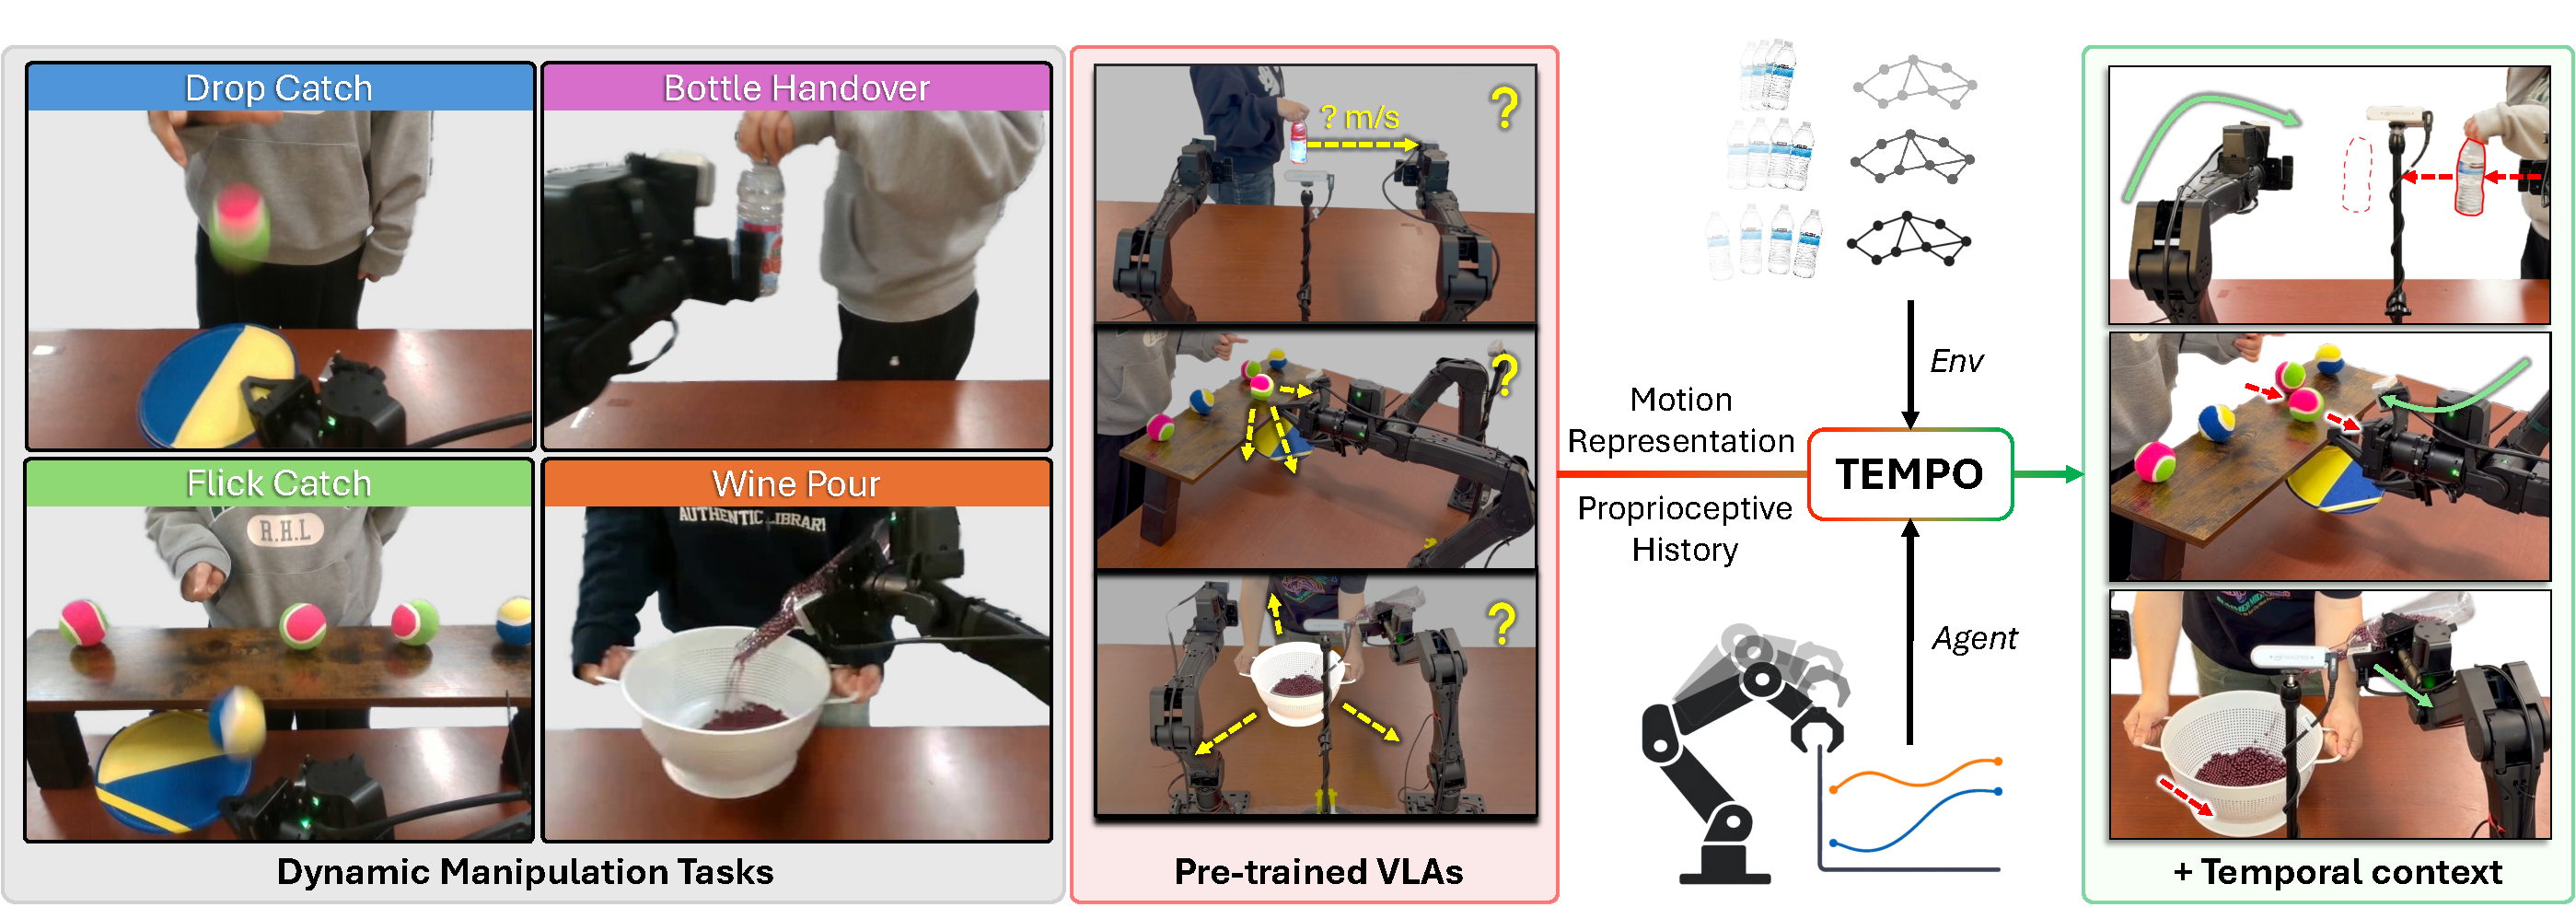
\includegraphics[width=\columnwidth]{2026-corl-unveil-template/figures/teaser.pdf}
	\caption{\textbf{\ours\ makes a pretrained VLA motion-aware.}
	Four dynamic tasks (\emph{left}) in which the target object
	is in motion throughout the episode.
	A standard VLA, conditioned on a single observation, cannot determine
	how the scene is evolving (\emph{center, red}; ``?\,m/s'') and cannot
	disambiguate perceptually identical observations that arise at
	different phases of the same task, producing failed grasps and
	mistimed actions.
	\ours\ resolves both failure modes by augmenting the policy with two
	compact signals: \TEMPOMOT, a motion representation from a frozen
	video foundation model, and \TEMPOACT, a compact proprioceptive
	history providing subtask context.
	Together they enable reliable task completion across all four tasks
	(\emph{right, green}).}
	\label{fig:teaser}
\end{figure}
We evaluate on a bimanual platform across four dynamic tasks designed to expose each failure mode in isolation and combination: Bottle Handover, Drop Catch, Flick Catch, and Wine Pour. On tasks where motion perception or state disambiguation is the limiting factor, \ours\ outperforms both asynchronous baselines: Bottle Handover improves from 44\% to 74\%, and \ours\ is the only system to complete the full versions of Wine Pour and Flick Catch, where both baselines score $0\%$ due to unresolved state aliasing. Results on Drop Catch further validate the framework: it is the one task where execution timing dominates over representation, and it is precisely where asynchronous inference shines, consistent with the complementary relationship we describe above~(\figref{fig:jittery}). Ablations and probing analyses confirm that each signal is individually necessary, relied upon at distinct moments (\TEMPOMOT\ during tracking, \TEMPOACT\ at commitment), and that the motion token encodes object velocity.

We argue that extending pretrained VLAs to dynamic settings is primarily a question of representation, not scale: the temporal context needed to act in a moving scene decomposes into two distinct signals, each tied to a distinct failure mode and independently verifiable. Our contributions are: (1) we identify and formalize two representational failure modes of single-frame VLAs in dynamic settings, \emph{motion ambiguity} and \emph{state aliasing}, and show that neither is a latency nor a capacity failure; (2) we address such failure modes and introduce two minimal plug-and-play inputs, \TEMPOMOT, an abstract past motion representation, and \TEMPOACT, a compact proprioceptive history, that together make any pretrained VLA motion-aware without extensive pretraining efforts; and (3) we release \benchname, an object-motion benchmark of over 50k frames of human-robot dynamic manipulation with per-frame object-velocity annotations, together with a multiple-choice variant in the format of MVBench~\cite{li2024mvbench} and VLM4D~\cite{zhou2025vlm4d} with object moving direction and motion magnitude question, targeted at evaluating motion understanding in VLMs and VLAs.



%===============================================================================

% \section{Related Work}
% \label{sec:related-work}

% \noindent\textbf{Dynamic Tasks for Robotics.}
% Dynamic tasks have been a long-studied problem in the robotics field for more than a decade, and have produced plentiful impressive results on complex, fast-moving tasks: Table Tennis~\cite{tabletennis, mstennis}, Object Tossing~\cite{zeng2020tossingbot, flingbot, dynamichandover}, and Object Catching~\cite{catchit, dynamichandover}. However, prior work mostly focuses on explicitly tracking and modeling object physics and translating it into the corresponding robot actions. Although this line of work achieves impressive results, it is far from generalizable: each system is typically an entire pipeline designed for a single task and does not transfer to other dynamic tasks. This brings us to Vision-Language-Action models, which are pretrained on much larger datasets and designed to be generalizable.

% \noindent\textbf{Vision-Language-Action Model for Dynamic Tasks.} Vision-Language-Action (VLA) models have recently seen significant advances in the robotics field. Many state-of-the-art models can be fine-tuned in dozens of GPU-hours to perform complex, long-horizon tasks~\cite{openvla, rt2, octo, vla-adapter, pi05}. Within this fast-moving field, dynamic tasks stands apart from typical VLA benchmarks: they often involve a constantly evolving environment and moving objects, and require the VLA to react in order to succeed. So far, research has focused on reducing the delay between action-chunk executions, known as asynchronous inference, as detailed below.

% \noindent\textbf{Asynchronous Inference for Dynamic Tasks.} 
% In an effort to adapt VLA models to dynamic tasks, research began exploring ways to cut the inference delay between action-chunk executions~\cite{leave_no, rtc,smolvla}. SmolVLA~\cite{smolvla} introduced an asynchronous-inference pipeline that begins policy inference preemptively, before the current action chunk finishes executing. This hides the idle gap in which a standard VLA waits for the next chunk to be predicted after the current one ends. However, the observation that launches inference is stale by the time the new chunk begins, and this mismatch produces jittery motion at chunk transitions. RTC~\cite{rtc} and VLASH~\cite{vlash} each introduce a way to smooth this transition, followed by many other works~\cite{dynamicvla, f2fap}. However, to date, no VLA has addressed a crucial aspect of dynamic tasks: motion understanding.


% %===============================================================================


\section{Related Work}
\label{sec:related-work}

\noindent\textbf{Dynamic Tasks for Robotics.}
Dynamic manipulation has a long research history, with compelling results on table tennis~\cite{tabletennis, mstennis}, object tossing~\cite{zeng2020tossingbot, flingbot}, and aerial catching~\cite{catchit, dynamichandover}. These systems achieve strong performance by explicitly modeling object physics and designing task-specific controllers, but each is an end-to-end pipeline for a single scenario that does not transfer to other tasks. In contrast, pretrained VLA models~\cite{brohan2022rt, driess2023palm, openvla, rt2, octo, pi0, pi05} generalize across tasks without per-task engineering; extending them to dynamic settings is the focus of this work.

\noindent\textbf{Asynchronous Inference for Dynamic Tasks.}
A prominent line of work addresses the \emph{execution timing} problem: inference latency of VLA models causes the executed chunk~\cite{chi2023diffusion,zhao2023act} to be conditioned on a stale observation. SmolVLA~\cite{smolvla}, RTC~\cite{rtc}, VLASH~\cite{vlash}, and Leave No Observation Behind~\cite{leave_no} each reduce or correct for this staleness. DynamicVLA~\cite{dynamicvla} co-designs a compact VLA architecture with continuous inference and latent-aware streaming for lower-latency dynamic control. F2F-AP~\cite{f2fap} takes a different route within the same problem: it predicts optical flow to synthesize an anticipated future frame, giving the policy visual context that compensates for latency. \ours\ is orthogonal to all of these: asynchronous inference addresses \emph{when} a prediction is applied; \ours\ addresses \emph{what} the policy is conditioned on. Even with a fresh or anticipated observation, a snapshot cannot encode how the scene is evolving or disambiguate sequential task phases. We build \ours\ on the asynchronous backbone of~\cite{vlash} so our experiments directly isolate the contribution of motion-aware representation; the two approaches are complementary and can be combined.

\noindent\textbf{Visual and Visuomotor Representations in Robot Learning.}
A parallel line of work asks what \emph{static} representation a policy should be conditioned on. Visual pretraining from large-scale ego-centric or robot video~\cite{r3m, mvp, sensorimotor} learns transferable features~\cite{data4robotics} before any downstream policy fine-tuning. RoboAffordances~\cite{roboaffordances} instead distills task-agnostic affordance priors from human videos, and HPT~\cite{hpt} scales pretraining across heterogeneous embodiments. UVT~\cite{uvt} and Anchor-Align~\cite{anchoralign} shape the training \emph{signal} rather than the input. All of these methods condition the policy on a single frame. \ours\ instead supplying the temporal context that no single frame can carry.


%===============================================================================


\section{Motion Ambiguity and State Aliasing}
\label{sec:diagnosis}

As briefed in \cref{sec:introduction}, we observe two dominant failure modes recent VLA encounters when trained on dynamic tasks, both stemming from a Markovian assumption shared by every pretrained VLA today, where the current observation is treated as a sufficient context for inferring action. We illustrate each on our four dynamic tasks (setup in \cref{sec:exp-setup}).

\begin{figure}[!t]
	\centering
	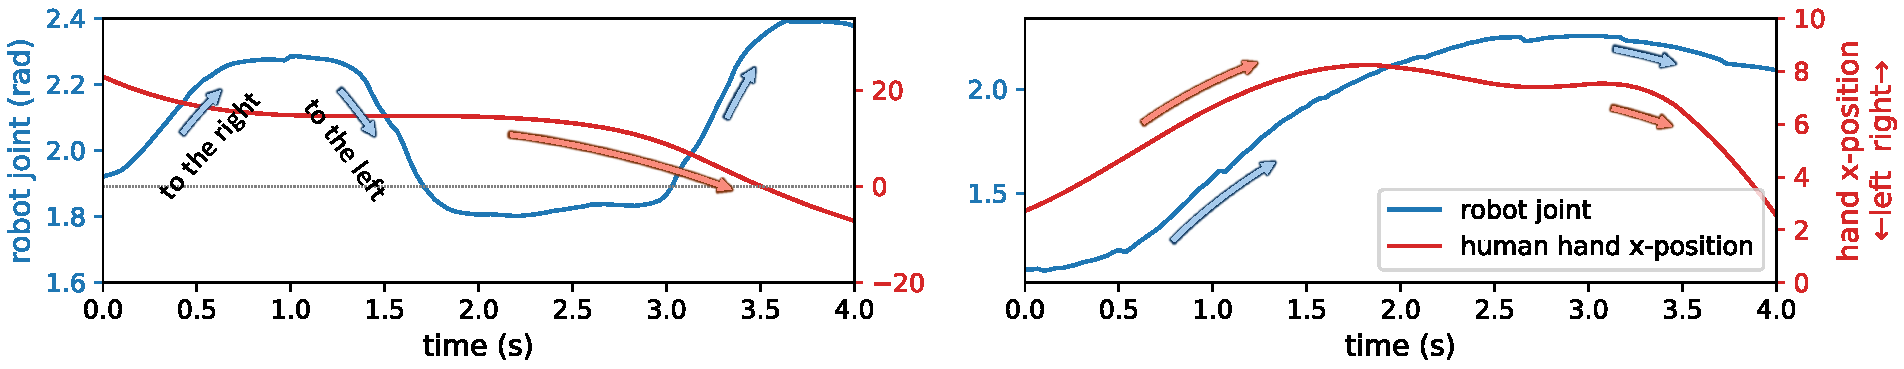
\includegraphics[width=0.9\columnwidth]{2026-corl-unveil-template/figures/jittery.pdf}
	\vspace{-1em}
	\caption{\textbf{Robot joint action (blue) does not track the human hand (red).} Side-by-side comparison of a Drop Catch rollout from the baseline (VLASH, left) and \ours~(right). The baseline oscillates left-to-right continuously while the human hand moves in a single direction, whereas \ours~closely tracks the hand.}
	\label{fig:jittery}
\end{figure}

\noindent\textbf{Motion ambiguity.}
A policy $\pi(o_t)$ conditioned on the current frame observes where objects are, but not where they are going. Recent works on dynamic tasks all focus on reducing inference latency, which lets $\pi$ act on a more recent observation, but does not inform the policy of object motion. \figref{fig:jittery} shows the resulting behavior on Drop Catch: when the policy is supposed to shadow human hand motion, the VLASH~\cite{vlash} policy instead produces actions that oscillate left-to-right. The same representational gap is also evident in our motion probe study in \cref{para:motion_probe}: linearly decoding object velocity from each baseline collapses on tasks where object motion is the only cue, with $R^2 \le 0.03$ on Flick Catch and $\le 0.09$ on Wine Pour (\cref{tab:motion_probe}). The policy has no basis for anticipating where a moving target will be.

\begin{wraptable}{r}{0.45\columnwidth}
\centering
\small
\setlength{\tabcolsep}{4pt}
\begin{tabular}{lcc}
\toprule
Method & Flick Catch & Wine Pour \\
\midrule
RTC~\cite{rtc} & 0\% & 0\% \\
VLASH~\cite{vlash} & 0\% & 0\% \\
\ours~(Ours) & \textbf{68\%} & \textbf{97.6\%} \\
\bottomrule
\end{tabular}
\caption{\textbf{Success on the untrimmed Flick Catch and Wine Pour}, where each episode retains the release-and-retract phase that produces state aliasing. Both asynchronous baselines fail every rollout; \ours\ completes the task by using \TEMPOACT\ to disambiguate phases the current frame cannot.}
\label{tab:state_alias}
\end{wraptable}

\noindent\textbf{State aliasing.}
A second failure mode arises from task structure and persists in the absence of motion. Multi-stage tasks force the policy to produce opposite actions from visually near-identical moments. For example, reaching for a plate at the start of a task and releasing it and pulling the gripper back look nearly the same from the head camera, but the corresponding future actions are opposite. The policy then hesitates between the two options: the gripper commits to neither, and the task fails to advance. Trained on the original Wine Pour and Flick Catch tasks, both asynchronous baselines fail every rollout ($0/50$; \cref{tab:state_alias}). To obtain nonzero baseline numbers for the main results in \cref{tab:success_rates}, we manually remove aliased state by trimming the release-and-retract phase from every training episode. Having to remove this segment at all is itself evidence of the failure for our baseline models.

\noindent\textbf{What the two failures require.}
Both failures come down to the same gap: a single frame carries no temporal context. To perceive scene motion, the policy needs a signal built from recent observations; to tell task phases apart, it needs a signal built from its own recent actions. Both signals summarize data the policy is already receiving at inference time.

%===============================================================================


\section{\methodname}
\label{sec:method}

\begin{figure}[t]
	\centering
	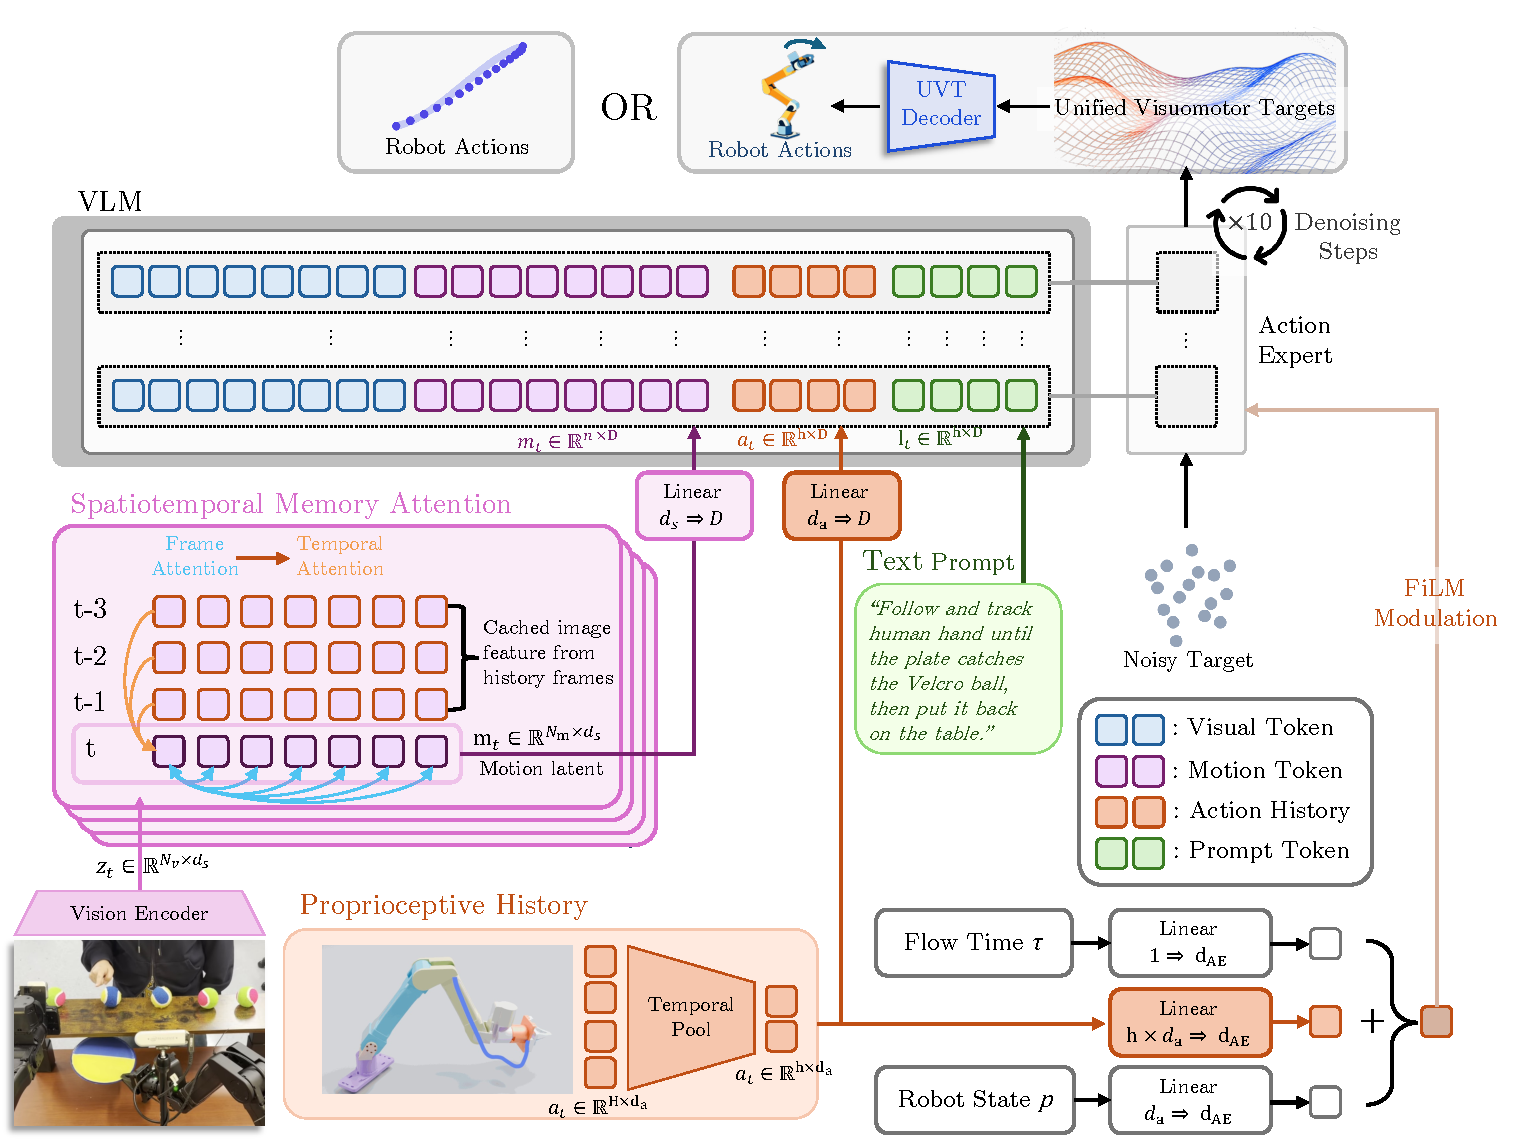
\includegraphics[width=0.95\columnwidth]{2026-corl-unveil-template/figures/tempo_main.pdf}
	\vspace{-0.6em}
	\caption{\textbf{\ours\ architecture.} \ours\ augments a pretrained VLM-based policy with two temporal inputs. \TEMPOMOT\ cross-attends the current frame's patch features $\mathbf{f}_t$ against a streaming cache $\mathcal{F}_t$ of features from the preceding $W-1$ frames, producing a motion code $\mathbf{m}_t$ that encodes scene dynamics. \TEMPOACT\ mean pools the robot's recent proprioceptive command history into $K$ fixed-size buckets, yielding a compact summary $\mathbf{c}_t$. Both signals attach to the pretrained backbone with near-zero overhead: $\mathbf{m}_t$ and $\mathbf{c}_t$ are projected to the VLM's token dimension and appended to its prefix, and $\mathbf{c}_t$ additionally conditions the action expert via an AdaRMS residual.}
	\label{fig:method}
\end{figure}
% we can add an optional module uvt 

\ours\ supplies the two temporal signals that \cref{sec:diagnosis} identifies as missing: \TEMPOMOT, a motion encoder that summarizes recent scene dynamics, and \TEMPOACT, a compact proprioceptive history. Both attach to a pretrained VLA with near-zero overhead (\figref{fig:method}).


\vspace{-0.3em}
\subsection{\TEMPOMOT: Captures Object and Scene Dynamics}
\TEMPOMOT\ summarizes recent visual dynamics by cross-attending the current frame against a rolling cache of past frames (\figref{fig:method}). Let $\mathbf{f}_\tau$ denote the patch features of observation $o_\tau$, extracted by $\phi$'s per-frame encoder. Over a streaming window of length $W$, we maintain a cache $\mathcal{F}_t = \{\mathbf{f}_\tau\}_{\tau=t-W+1}^{t-1}$ of features from the preceding $W-1$ frames, populated incrementally so that each $\mathbf{f}_\tau$ is computed exactly once and reused on subsequent steps at no additional cost. The motion code is then
\begin{equation}
\label{eq:tempomot}
\mathbf{m}_t \;=\; \phi(o_{t-W+1:t}) \;=\; \operatorname{CrossAttn}\bigl(\mathbf{f}_t,\; \mathcal{F}_t\bigr),
\end{equation}
with the current-frame features $\mathbf{f}_t$ as queries and historical visual features as keys and values.

\begin{wraptable}{r}{0.42\columnwidth}
\centering
\vspace{-\baselineskip}
\small
\setlength{\tabcolsep}{4pt}
\begin{tabular}{lc}
\toprule
Motion encoder $\phi$ & Handover \\
\midrule
SAM~2.1-Tiny~\cite{sam2} (default) & \textbf{74\%} \\
Reducio~\cite{reducio}       & \textbf{76\%} \\
VidTwin~\cite{vidtwin}       & 60\% \\
VideoLaVIT~\cite{videolavit} & 52\% \\
\bottomrule
\end{tabular}
\caption{\textbf{Swapping the motion encoder $\phi$} keeps Bottle Handover success comfortably above the VLASH baseline ($38\%$).}
\label{tab:encoder_swap}
\end{wraptable}
We instantiate $\phi$ with a frozen pretrained video foundation model, used off-the-shelf without motion-specific fine-tuning; SAM~2.1-tiny~\cite{sam2} is our default. The choice is flexible: any video encoder whose features separate motion from appearance can serve as $\phi$. \figref{fig:ball_velocity_probe} shows that object velocity is linearly decodable from $\mathbf{m}_t$ computed from different video encoders, substantially outperforming a position-only baseline, across several encoder families, and \cref{tab:encoder_swap} confirms the same conclusion at the task level: swapping $\phi$ across four video foundation models keeps Bottle Handover success in the $52$–$76\%$ range, all well above the VLASH baseline. Reducio slightly exceeds our SAM default; we still adopt SAM~2.1-Tiny for the streaming speed required at real-time control rates (\tabref{tab:latency_comparison}).

\vspace{-0.3em}
\subsection{\TEMPOACT: Resolves State Aliasing}
Where \TEMPOMOT\ captures how the scene is moving, \TEMPOACT\ captures what the robot has been doing. A compact summary of recent proprioceptive history gives the temporal context for the robot policy to commit to the correct task phase. Without resolving state aliasing, the policy averages over multiple valid actions for the same observation, often producing indecisive behavior (e.g., pausing) or oscillating between conflicting actions, as seen in our baseline rollouts (\cref{fig:ambiguity}).

Raw proprioceptive history is long, high-frequency, and largely redundant, so we compact it into a fixed-size summary $\mathbf{c}_t$ (\TEMPOACT). Let the proprioceptive command at time $\tau$ be $q_\tau\in\mathbb{R}^{d_q}$. We consider the most recent $H$ commands preceding time $t$, partition them into $K$ contiguous temporal buckets $B_1,\ldots,B_K$ of equal length $L$ (so that $H=KL$), ordered from oldest to newest, and summarize each bucket by its mean:
\begin{equation}
\label{eq:joint-compaction}
\mathbf{c}_t=\bigl(\bar q^{(1)}_t,\dots,\bar q^{(K)}_t\bigr),\qquad
\bar q^{(k)}_t=\frac{1}{L}\sum_{\tau\in B_k} q_\tau\in\mathbb{R}^{d_q},\qquad
q_\tau:=0\ \text{for }\tau<\text{episode start}.
\end{equation}
% \vspace{-0.5em}

We use $K=10$ buckets, each averaging $L=30$ consecutive commands. Buckets that fall entirely before the episode start are marked with a pad flag. The resulting representation $\mathbf{c}_t\in\mathbb{R}^{K\times d_q}$ always contains $K$ tokens, regardless of how much history it summarizes. Extending the temporal horizon only changes the bucket length $L$, not the number of tokens. This simple, parameter-free aggregation preserves a coarse trend of robot's recent motion while adding negligible computational overhead.

\vspace{-0.3em}
\subsection{Plug-and-Play Temporal Integration}
We add the two signals to a pretrained VLA while keeping the pretrained backbone largely intact (\figref{fig:method}). We build on VLASH's asynchronous-inference pipeline~\cite{vlash} as the backbone, though our additions are agnostic to this choice. $\mathbf{m}_t$ is projected to the VLM's token dimension and appended to its prefix alongside the current multi-view observation and the language instruction. The action expert reads the resulting VLM prefix through the cross-attention layers. 

The $K$ bucket tokens of $\mathbf{c}_t$ are used in two ways. First, they are projected into VLM's prefix tokens dimension and appended to the VLM token stream, allowing the multimodal prefix to include the robot's recent proprioceptive history. Second, the same bucket sequence is flattened and passed through a conditioning MLP to produce an AdaRMS residual for the action expert, modulating the denoising process directly. 

Together, the two temporal signals provide complementary temporal contexts to the VLA.
The added conditioning path is zero-initialized, so the pretrained policy's behavior is preserved at the start of fine-tuning. Flow-matching loss is unchanged, and \ours\ adds only 2M~($0.08$\%) parameters.

\vspace{-0.3em}
\subsection{Real-Time Deployment via Parallel Encoding}
\begin{wraptable}{r}{0.40\columnwidth}
\centering
\vspace{-\baselineskip}
\small
\setlength{\tabcolsep}{4pt}
\begin{tabular}{lc}
\toprule
\textbf{Method} & \textbf{Median} \\
\midrule
VLASH~\cite{vlash}          & 33.8 ms \\
RTC~\cite{rtc}              & 127.7 ms \\
\ours~(Ours)                & 35.3 ms \\
\bottomrule
\end{tabular}
\caption{Inference latency comparison across methods.}
\label{tab:latency_comparison}
\end{wraptable}
\TEMPOMOT\ is encoded in a dedicated background thread, decoupled from the control loop: the motion encoder consumes camera frames at sensor rate ($\sim$11\,ms per frame on an NVIDIA RTX PRO 6000) and continuously updates the latest motion token, which the policy reads at each control step. The only overhead the policy pays is about 1.5\,ms for attending to the extra token (35.3\,ms vs.\ 33.8\,ms median forward time; \tabref{tab:latency_comparison}), versus approximately 128\,ms per chunk for the asynchronous baseline RTC~\cite{rtc}. Because $\phi$ operates over a fixed-size streaming window, its per-frame cost stays constant regardless of history length, so \ours\ adds motion awareness without impacting the policy's control rate.

%===============================================================================



\section{Experiments}

\begin{table}[h]
\centering
\small
\begin{tabular}{lccccc}
\toprule
Method & Bottle Handover & Drop Catch & Flick Catch & Wine Pour & Average \\
\midrule
% $\pi_{0.5}$ & & & & \\
RTC~\cite{rtc} & 44\% & 80\% & 48\% & 80.8\% & 63.2\% \\
VLASH~\cite{vlash} & 38\% & 38\% & 20\% & 94.0\% & 47.5\% \\
\ours~(Ours)  & 74\% & 66\% & 66\% & \textbf{98.1\%} & 76.0\% \\
TEMPO+UVT~\cite{uvt} & \textbf{88\%} & \textbf{88\%} & \textbf{76\%} & 96.7\% & \textbf{87.2\%}\\
\bottomrule
\end{tabular}
\vspace{1em}
\caption{\textbf{Success rates across the four dynamic tasks.} Each
entry is the percentage of $50$ real-world rollouts in which the policy completes
the task, evaluated under varied object speeds, appearances,
and approach directions. For Wine Pour task, instead of recording binary success or failure, we measure the percentage of the "wine" mass retained in the pot at the end of the pour.}
\label{tab:success_rates}
\vspace{-4mm}
\end{table}


\label{sec:experiments}



\subsection{Experimental Setup}
\label{sec:exp-setup}


\label{sec:setup}
\begin{figure}[!tbp]
	\centering
	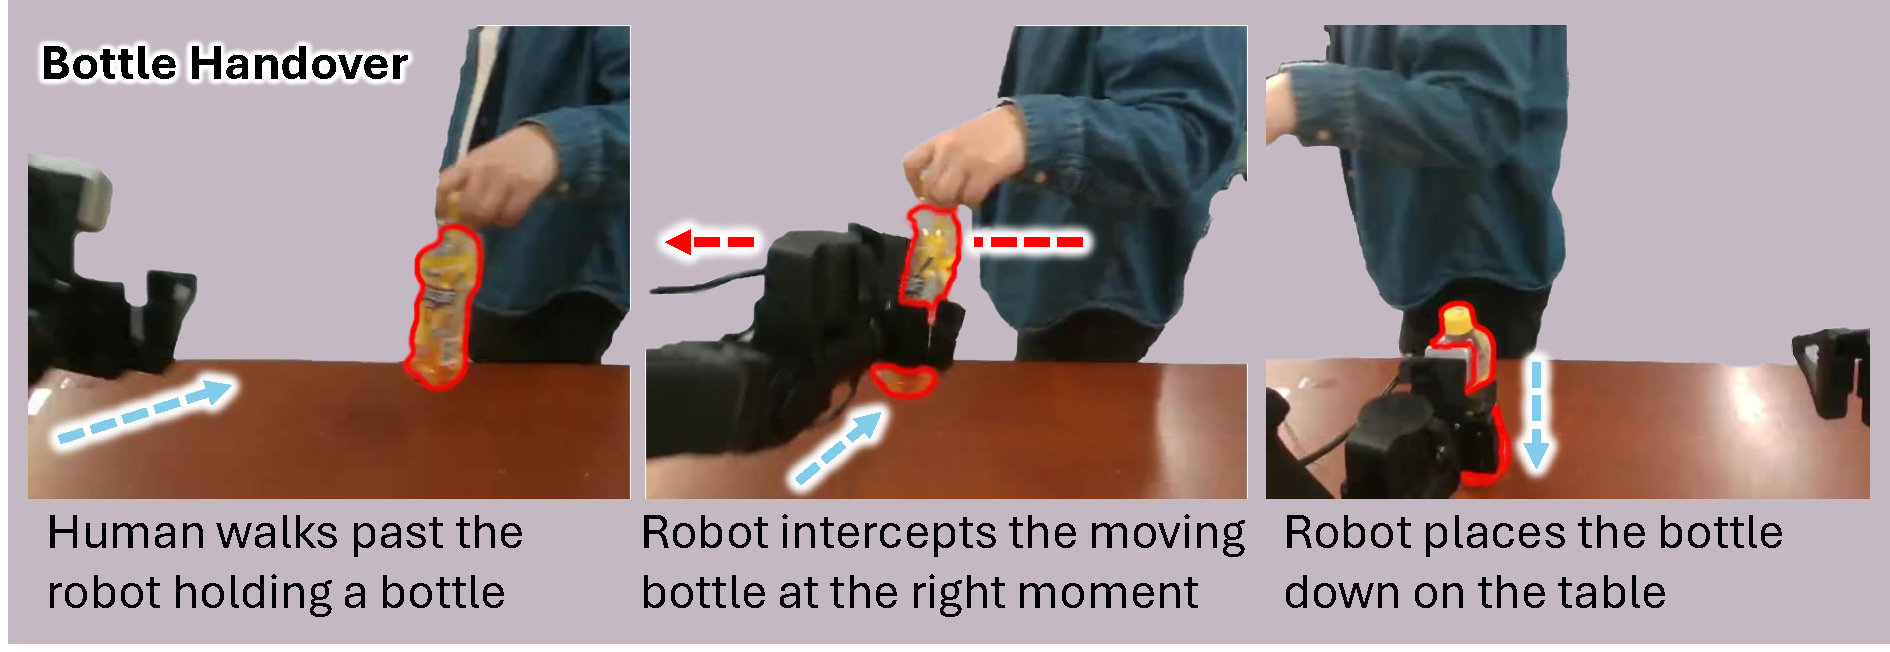
\includegraphics[width=0.5\columnwidth]{2026-corl-unveil-template/figures/handover.pdf}\hfill
	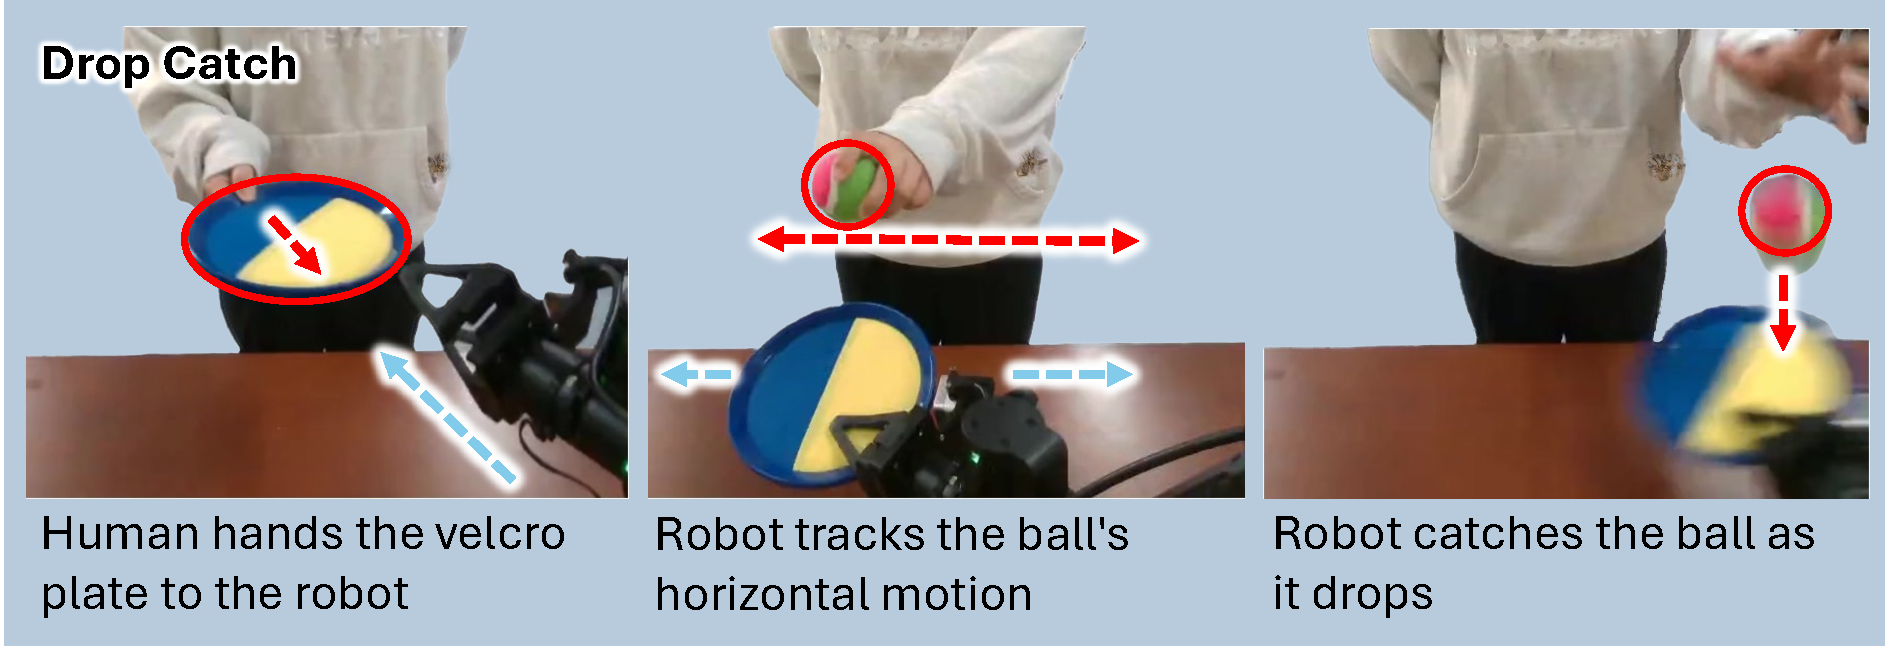
\includegraphics[width=0.5\columnwidth]{2026-corl-unveil-template/figures/drop.pdf}\\
	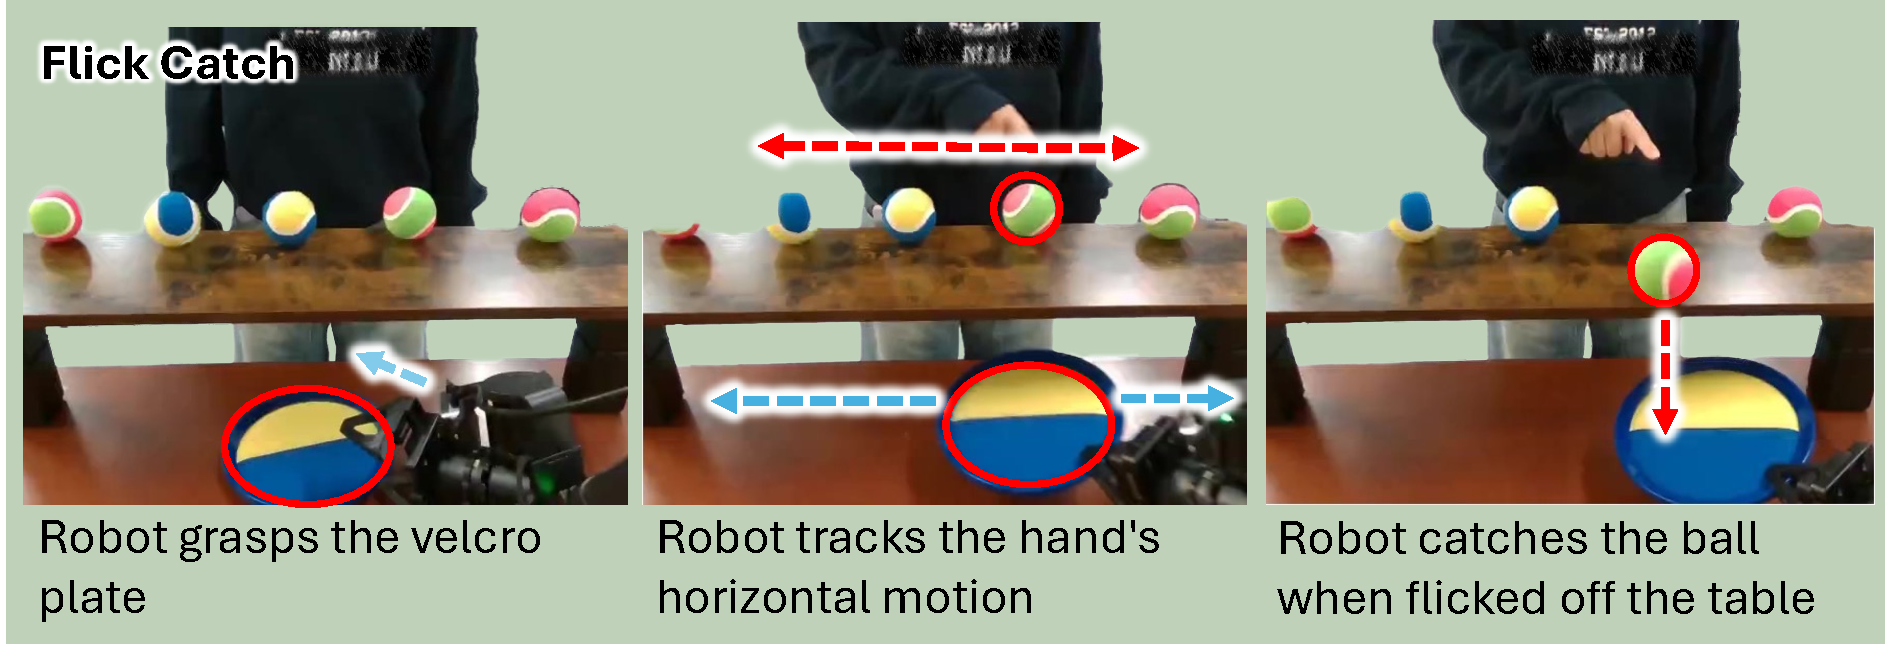
\includegraphics[width=0.5\columnwidth]{2026-corl-unveil-template/figures/flick.pdf}\hfill
	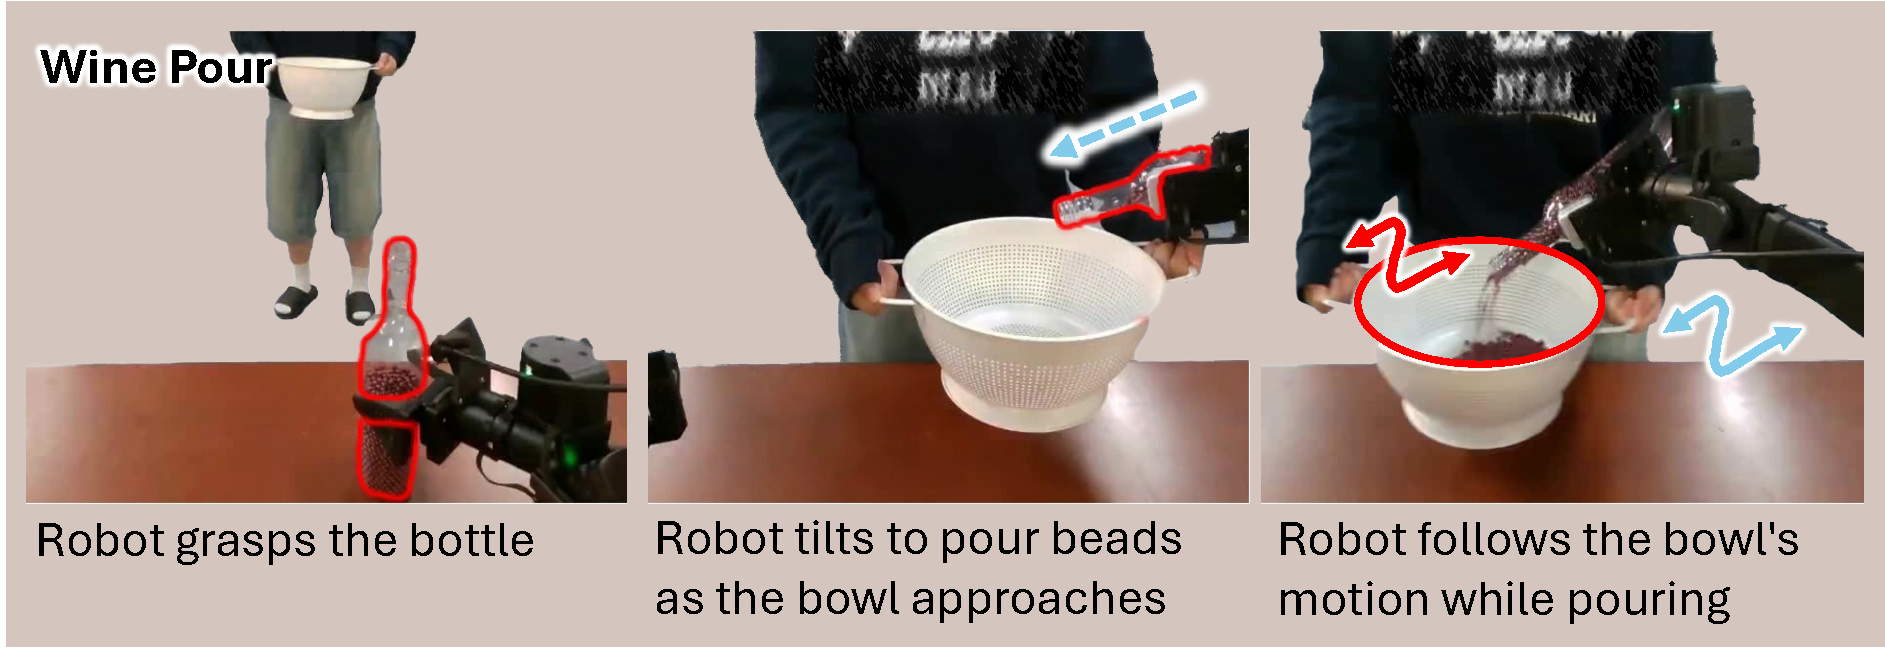
\includegraphics[width=0.5\columnwidth]{2026-corl-unveil-template/figures/pour.pdf}
	\caption{\textbf{Task Setup.} We benchmark all models across four comprehensive dynamic tasks.}
	\label{fig:tasks}
\end{figure}

We design four tasks to expose the two ambiguities identified in \cref{sec:introduction}: motion ambiguity and state aliasing. We ask whether \ours\ resolves each kind of ambiguity through \TEMPOMOT\ and \TEMPOACT. We compare \ours\ against two state-of-the-art asynchronous baselines designed for responsive task execution, RTC~\cite{rtc} and VLASH~\cite{vlash}. For Wine Pour and Flick Catch, both baselines collapse to $0\%$ on the full task because the release-and-retract phase is perceptually aliased with reaching. As a result, a baseline that sees the gripper near the bottle or plate cannot tell whether to grasp or withdraw and oscillates between the two (more detailed visualization and analysis in \cref{app:failure}). To avoid a trivial comparison, we report quantitative results on a trimmed version that removes the release-and-retract phase, eliminating this artifact. We emphasize that \ours\ disambiguates these phases through \TEMPOMOT\ and \TEMPOACT, so the gain in \cref{tab:success_rates} is a lower bound on \ours's full-task advantage. For qualitative rollouts of the baselines' complete failure and \ours's behavior, please see our project webpage and \cref{app:failure}.


\noindent\textbf{Task properties.}\label{sec:task_properties} Each of the four tasks is dynamic and shares four properties that a current-frame observation alone cannot resolve.
  \textbf{(P1)} The target object is moving at varying motion. Therefore, reacting based on the current snapshot alone is inaccurate in both position and timing.
  \textbf{(P2)} The relevant target shifts during the episode. As a result, the policy must redirect its attention to whichever object currently matters.
  \textbf{(P3)} Each task decomposes into a sequence of subtasks (approach, grasp, track, release), and the correct next action depends on which subtask has already been completed.
  \textbf{(P4)} The policy faces state ambiguity. From the current frame alone, multiple next actions are plausible, and a perceptually identical state may demand opposite actions depending on what has come before. 

   
\textbf{Bottle Handover (P1).}~The robot intercepts a bottle from a human walking by from either direction. We vary the walking speed, bottle's height, and holding pose across episodes, so the policy must estimate the bottle's velocity to time and place the grasp correctly.
\\\textbf{Drop Catch (P1, P3).}~The robot catches a ball dropped by a horizontally moving human hand. Each episode begins with the human handing a Velcro plate to the robot, after which the robot tracks the human’s hand laterally before catching the released ball. This task includes a moving dynamic object (P1) and multiple sequential subtasks (P3).
\\\textbf{Flick Catch (P1--P4).}~Several Velcro balls rest on a long horizontal platform. The robot first picks up a Velcro plate from the table (P3). A human hand then hovers over the balls and, at a random time, flicks one off the platform. The robot must first track the hand, then switch to tracking the released ball to catch it in time (P2, P1). Because the robot picks up and later places down the plate at the same location, the pick-up is perceptually aliased with the subsequent drop-off (P4), making this the most challenging of the four tasks.
\\\textbf{Wine Pour (P1--P4).}~The robot pours beads, an alternative to wine, into a pot that the human moves around. The task decomposes into three subtasks (P3): pick up the bottle from the table, pour while tracking the pot movement, and put the bottle back down. Pick-up and put-down produce visually similar states yet require opposite actions, producing state aliasing (P4). Once pouring begins, the target shifts from the bottle to the pot (P2), whose motion must be tracked (P1). Since every rollout inevitably spilled some beads, this task's success is determined by the percentage of beads' mass retained in the pot at the end of the pour.


\subsection{Experimental Results}
\label{sec:quant}

\begin{figure}[!tbp]
	\centering
 	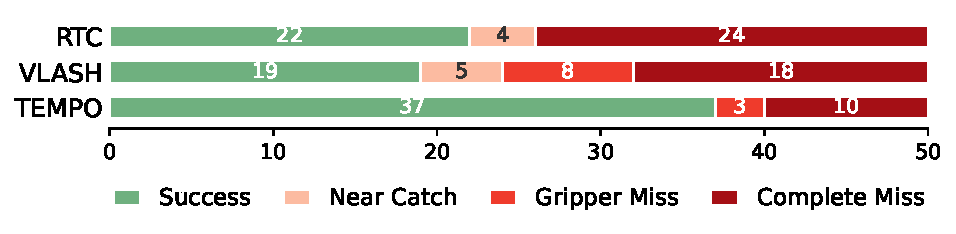
\includegraphics[width=0.8\columnwidth]{2026-corl-unveil-template/figures/failure_modes.pdf}
    \vspace{-1em}
	\caption{\textbf{Failure-mode breakdown on Bottle Handover}, we categorized and visually examined each episode in deployment rollouts and attributed each model's failure to different categories.}
	\label{fig:failure_modes}
\end{figure}

\noindent\textbf{Success Rate on Dynamic Tasks.}
As shown in \cref{tab:success_rates}, we extensively compare our method against each of the SOTA asynchronous VLA models. For each task, we calculated success rate for each model based on 50 trials following the evaluation protocol established under \cref{sec:setup}. On simpler tasks like Drop Catch, \ours\ achieves a competitive success rate compared to RTC, while VLASH frequently overshoots the human motion and misses the dropped ball. Across the remaining tasks where the object motion is more uncertain or the object of interest shifts, \ours\ consistently outperforms both baselines, including $+36\%$ on Bottle Handover, $+4.1\%$ on Wine Pour, and $+46\%$ on Flick Catch. We observed closer tracking of the human hand by the robot gripper in Drop Catch and Flick Catch, as well as more precisely timed grasps in Bottle Handover.




\noindent\textbf{Failure mode analysis.}
A single success rate hides \emph{why} a policy fails, so we visually examined all
$50$ rollouts of every model on Bottle Handover and labeled each as a success or
one of three failure modes (\figref{fig:failure_modes}). The dominant failure for both baselines is \emph{Complete Miss}, where the arm reaches toward the wrong place and misses the bottle entirely, indicating that the policy mispredicts where the moving bottle will be. VLASH and RTC commit $18$ and $24$ Complete Misses respectively, while the timing-related \emph{Gripper Miss} and the near-success \emph{Near Catch} are comparatively rare. By conditioning on recent motion, \ours\ cuts Complete Misses to $10$ and raises success from $19$ (VLASH) and $22$ (RTC) to $37$ out of $50$. Although both asynchronous pipelines significantly reduce inference delay, a lack of motion understanding still hurts dynamic-task performance.


\begin{wraptable}{r}{0.42\columnwidth}
\centering
\vspace{-\baselineskip}
\small
\setlength{\tabcolsep}{4pt}
\begin{tabular}{lcc}
\toprule
VLA backbone & Base & + \ours \\
\midrule
$\pi_{0.5}$~\cite{pi05}   & 26\% & \textbf{56\%} \\
RTC~\cite{rtc}            & 44\% & \textbf{80\%} \\
VLASH~\cite{vlash}        & 38\% & \textbf{74\%} \\
\bottomrule
\end{tabular}
\caption{\textbf{\ours\ is plug-and-play across VLA backbones.} Adding \TEMPOMOT\ and \TEMPOACT\ improves Bottle Handover on all backbones, including the non-asynchronous $\pi_{0.5}$.}
\label{tab:backbone_integration}
\end{wraptable}
\noindent\textbf{Plug-and-play across VLA backbones.}
The two temporal inputs of \ours\ are not backbone-specific. We attach the same \TEMPOMOT\ and \TEMPOACT\ to two additional pretrained VLAs, $\pi_{0.5}$~\cite{pi05} (non-asynchronous) and RTC~\cite{rtc}, and retrain each on the same Bottle Handover demos. Every backbone we tried improves substantially: $\pi_{0.5}$ from $26\%$ to $56\%$, RTC from $44\%$ to $80\%$, and VLASH from $38\%$ to $74\%$ (\cref{tab:backbone_integration}). \ours\ helps both asynchronous and non-asynchronous backbones, indicating that motion-aware perception is a general upgrade rather than a VLASH-specific effect.


\noindent\textbf{Extending TEMPO with a compact training target.}
With \ours\ closing the input-side gap, a natural line of question being whether anything remains on the output side. Our prior work, Unified Visuomotor Target (UVT)~\cite{uvt}, argues that it does: VLAs are typically trained to predict raw joint-position chunks, which are high-dimensional and jitter-prone, and swapping this target for a compact motion primitive aligned with object motion tightens the target the policy has to learn. Since \ours\ and UVT act on different sides of the policy, they combine without redundancy: \ours+UVT achieves the highest overall success rate in \cref{tab:success_rates} and outperforms baselines on $3$ of the $4$ tasks, further pushing dynamic task performances.


\section{Analysis and Ablations}
\label{sec:ablation}
% Commented out: fig:attention (attention-mass visualization). The
% qualitative attention story was largely a narration of the figure
% and correlational; the causal input-ablation MSE curves in
% app:input_ablation carry the 'each signal matters at a different
% moment' claim more sharply.
\iffalse
\begin{figure}[t]
	\centering
	\includegraphics[width=0.8\columnwidth]{2026-corl-unveil-template/figures/attention_shrink.pdf}
	\vspace{-1em}
    \caption{\textbf{The policy attends to \TEMPOMOT\ and \TEMPOACT\ at different stages of the task.} \TEMPOMOT\ attention peaks when the human hand starts moving, whereas \TEMPOACT\ attention peaks during fast hand following.}
	\label{fig:attention}
\end{figure}
\fi



% Having shown that \ours\ outperforms recent VLA baselines on dynamic tasks that target execution latency rather than motion perception (\tabref{tab:success_rates}), we now turn to \emph{why}. Here we show that conditioning on two signals, the global object motion~(\TEMPOMOT) and the robot's joint history~(\TEMPOACT), is crucial for addressing two ambiguities: motion and state.

% We analyze along three axes.
% To show that both \TEMPOMOT~and \TEMPOACT~ are crucial for dynamic tasks, we propose three questions:
  % \textbf{(i) Why these two signals?} The structure of dynamic tasks that \TEMPOMOT\ and \TEMPOACT\ carry information that the current frame alone cannot provide.
  % \textbf{(ii) How does the policy uses both signals?} Action Expert (AE) transformer attention mass (\figref{fig:attention}) and per-frame ablation MSE (\figref{fig:attention_mse}) shows that \ours\ relies on \TEMPOMOT\ and \TEMPOACT\ at different moments, and that removing either causes the policy to revert to jittery and reactive behavior (\figref{fig:jittery}).  
  % \textbf{(iii) But what does \TEMPOMOT\ actually encode?}A linear probe of \TEMPOMOT\ against \llm{semi-automated annotation of object velocity} confirms that object motion is represented in the token.


Having shown \ours\ outperforms recent VLA baselines on dynamic tasks, we now turn to \emph{why}. We evaluate whether the policy relies on \TEMPOMOT\ and \TEMPOACT\ at the task stages where their corresponding ambiguities arise, using single-signal ablations and hidden-state probing.

% Commented out: attention-mass paragraph accompanying fig:attention.
% It was largely a narration of the figure and did not add a claim
% beyond what tab:input_ablation and app:input_ablation already carry.
\iffalse
In \figref{fig:attention}, we visualize how strongly the action expert emphasizes the two temporal signals over time. We investigate a representative episode on one of our hardest tasks, Flick Catch, and plot the attention mass that our model places on \TEMPOMOT\ and \TEMPOACT\ over the course of the episode. The \TEMPOMOT\ signal is emphasized as the human hand starts moving, which corresponds to major movement in the observation. \TEMPOACT\ then steadily gains more attention mass during the hand-following phase and drops back down after the ball is successfully caught. The same pattern generalizes across rollouts. Dropping \TEMPOMOT\ or \TEMPOACT\ during important phases significantly degrades action quality; see \cref{app:input_ablation} for the full ablation analysis.
\fi

  % Having motivated the design, we now show that the policy especially relies on \TEMPOMOT\ and \TEMPOACT~at certain crucial moments for the task. To verify, we examine when the policy attends to each signal and whether the two signals carry separable information by investigating what happens if we remove them.


\begin{wraptable}{r}{0.38\columnwidth}
\centering
\vspace{-\baselineskip}
\small
\setlength{\tabcolsep}{4pt}
\begin{tabular}{lc}
\toprule
Configuration & Handover \\
\midrule
\TEMPOACT\ only & 52\% \\
\TEMPOMOT\ only & 56\% \\
\ours\ (full)   & \textbf{74\%} \\
\bottomrule
\end{tabular}
\caption{\textbf{Both temporal signals contribute to the task.} Removing either \TEMPOMOT\ or \TEMPOACT\ reduces Bottle Handover success; the two together outperform either alone.}
\label{tab:input_ablation}
\end{wraptable}
\noindent\textbf{Each temporal signal is individually necessary.}
To verify that both \TEMPOMOT\ and \TEMPOACT\ carry non-redundant information for task success, we retrain \ours\ with each single signal removed and evaluate on Bottle Handover (\cref{tab:input_ablation}). Removing either signal substantially reduces success, and both single-signal variants still outperform the VLASH baseline (38\%), confirming that each temporal input is independently useful. Combining the two lifts success to $74\%$, above what either signal alone achieves. Each signal is also consulted at a distinct moment in the episode; see \cref{app:input_ablation} for the per-frame ablation MSE.


\noindent\textbf{Baseline hidden states lack motion on the hardest tasks.}
\label{para:motion_probe}
We test whether the trained policy encodes object motion by probing its hidden state at a fixed token position, following the same protocol as prior VLM probe works~\cite{zhao2024first, lu2025probing}. For each task we annotate the per-frame position of the object of interest and compute its pixel-space velocity, yielding an object-motion benchmark of over 50k annotated frames of human-robot dynamic manipulation that we release as \benchname, together with a multiple-choice variant in the format of MVBench~\cite{li2024mvbench} and VLM4D~\cite{zhou2025vlm4d}. Here we report the regression setting: we fit an MLP probe from each model's hidden state to the velocity and report $R^2$ (\cref{tab:motion_probe}).

\ours\ produces the strongest probe result on every row of \cref{tab:motion_probe}. Its hidden state decodes object velocity substantially better than the asynchronous baselines on the dynamic tasks where motion is the only cue (Flick Catch $R^2 = 0.57$ vs.\ ${\le}\,0.03$; Wine Pour $R^2 = 0.44$ vs.\ ${\le}\,0.09$), where the baseline probes collapse to near zero. Since RTC, VLASH, and \ours\ share the same $\pi_{0.5}$ backbone and pretraining, \ours's gain over the two is attributed to its motion-conditioned fine-tuning: \TEMPOMOT\ and \TEMPOACT\ leave a linearly-decodable motion signal in the hidden state that the other $\pi_{0.5}$-family backbones do not carry. We additionally ablate the choice of motion encoder, probing several video foundation models' latents for object velocity, in \cref{app:motion_encoder}.

\begin{table}[!t]
\centering
\small
\begin{tabular}{lccc}
\toprule
Task & RTC~\cite{rtc} & VLASH~\cite{vlash} & \ours \\
\midrule
Bottle Handover  & 0.46 & 0.43 & \textbf{0.52} \\
Drop Catch       & 0.31 & 0.28 & \textbf{0.33} \\
Flick Catch      & $-0.07$ & 0.03 & \textbf{0.57} \\
Wine Pour        & 0.06 & 0.09 & \textbf{0.44} \\
\midrule
Average          & 0.19 & 0.21 & \textbf{0.47} \\
\bottomrule
\end{tabular}
\vspace{1em}
\caption{\textbf{Motion probing of the trained VLA hidden state.} MLP probe on object velocity across our dynamic tasks ($R^2$). On Flick Catch and Wine Pour, where motion is the only usable cue, the asynchronous baselines' representations collapse to near zero while \ours's remains informative.}
\label{tab:motion_probe}
\vspace{-1em}
\end{table}

\label{sec:analysis}


%===============================================================================


% \section{Limitation}
% \label{sec:conclusion}

% In this work we have taken a step towards addressing the challenge of motion understanding in recent VLA models. While we largely improve success rates across the dynamic tasks and cut down the complete failures that result from poor understanding of scene motion, there are still a few cases where \ours~misses the object entirely; we leave this for future work. Because our approach is orthogonal to asynchronous inference, \ours~can be further improved as better asynchronous-inference methods are published.

% % I’d suggest we mention limitations in a style that
% % “we have taken a step towards adderssing and provide the structure necessary for advancing future work in it”
% % “… complement our proposed approach to help improve performance in future work.”
% % “Like methods in <method category>~\cite{}, \ours could benefit from …,”

% % But avoid getting unfairly evaluated by lazy LLMs, who will likely just latch on to an unhedged limitation.
% % Also avoid getting unfairly evaluated by lazy LLMs, “didn’t state any limitation or error analysis” and ding us for it.
% %===============================================================================
\section{Conclusion}
\label{sec:conclusion}

The gap between pretrained VLAs and dynamic manipulation is primarily representational: motion ambiguity and state aliasing each have a fix from representations already in wide use, and our failure mode breakdown (\figref{fig:failure_modes}) and ablation analyses (\secref{sec:ablation}) confirm that the two failures are separable and that each signal addresses its own. \ours\ implements this as two plug-and-play inputs with near-zero overhead; the gains on the untrimmed Wine Pour and Flick Catch, where asynchronous baselines score zero (\cref{tab:state_alias}), show that timing is not the bottleneck.

% A few limitations point to natural next steps. Our motion encoder operates on global scene flow; in highly cluttered scenes or under severe occlusion, the motion token may be noisy, and a more targeted tracking prior could help. Our experiments are conducted on a single bimanual platform, and broader validation across embodiments and task distributions remains important. Finally, because \ours\ is orthogonal to asynchronous inference and is built on top of~\cite{vlash}, it will benefit as faster and more accurate async methods appear.

%===============================================================================



\clearpage
% The acknowledgments are automatically included only in the final and preprint versions of the paper.
\acknowledgments{We thank CoRL reviewers and AC for their valuable feedback on improving papers, along with Basavasagar Patil for his careful reviews of the final draft of our paper.}

%===============================================================================


% no \bibliographystyle is required, since the corl style is automatically used.
\bibliography{example}  % .bib

\newpage
\appendix

% Renumber appendix figures and tables as A1, A2, ... and A1, A2, ...
\setcounter{figure}{0}
\setcounter{table}{0}
\renewcommand{\thefigure}{A\arabic{figure}}
\renewcommand{\thetable}{A\arabic{table}}

\section*{Appendix}
\addcontentsline{toc}{section}{Outline of the Appendix}

In this Appendix, we include extensions of analysis introduced in the main paper and additional technical details of our method, setup, and evaluation protocol. Qualitative rollouts, failure mode analysis, and more details are available on our project page: \url{https://tempo-robot.github.io/}.
\begin{itemize}
	\item \textbf{\cref{app:failure}, \emph{Additional Failure Mode Analysis}.} Supplements the trimming discussion in \cref{sec:exp-setup} and the success rates in \cref{tab:success_rates}. Explains why baselines collapse to $0\%$ on the original Flick Catch and Wine Pour, and reports \ours's performance on the untrimmed tasks (\cref{tab:state_alias}, \figref{fig:ambiguity}).
	\item \textbf{\cref{app:setup}, \emph{Experimental Setup Details}.} Supplements \cref{sec:exp-setup}. Lists the hardware platform, evaluation protocol, and training details for each method.
	\item \textbf{\cref{app:failure_breakdown}, \emph{Per-Task Failure Mode Breakdown}.} Supplements \cref{sec:quant} and the Bottle Handover breakdown in \figref{fig:failure_modes}. Extends the same per-rollout categorization to Flick Catch (\figref{fig:flick_failure}) and Drop Catch (\figref{fig:drop_failure}).
	\item \textbf{\cref{app:input_ablation}, \emph{Input Ablation}.} Supplements the single-signal ablations in \cref{sec:ablation}. Measures per-frame causal reliance on \TEMPOMOT\ and \TEMPOACT\ via input ablation MSE (\figref{fig:attention_mse}).
	\item \textbf{\cref{app:motion_encoder}, \emph{Motion Encoder Selection}.} Supplements the motion-encoder definition in \cref{sec:method} ($\phi$ in \TEMPOMOT). Justifies our choice of SAM~2.1-Tiny by linearly probing several candidate encoders for object velocity (\cref{fig:ball_velocity_probe}).
\end{itemize}


\section{Additional Failure Mode Analysis}
\label{app:failure}

\emph{Supplements the trimming discussion in \cref{sec:exp-setup} and \cref{tab:success_rates}; extends the state-aliasing evidence in \cref{sec:diagnosis}.} In our initial setup, every method was trained and evaluated on the complete, untrimmed versions of all four tasks. On Flick Catch and Wine Pour, both asynchronous baselines failed every rollout. The cause is state aliasing rather than reaction speed or accuracy: each episode contains a reach-out phase, in which the gripper approaches the velcro plate or the bottle, and a release-and-retract phase, in which the gripper recedes from the same object after grasping or pouring. The two phases produce visually near-identical observations yet demand opposite actions, and a single-frame policy has no cue to disambiguate them, so the gripper oscillates between extending toward and withdrawing from the object and never commits long enough to make progress (\figref{fig:ambiguity}; see qualitative rollouts on our project webpage).

\begin{figure}[h]
	\centering
	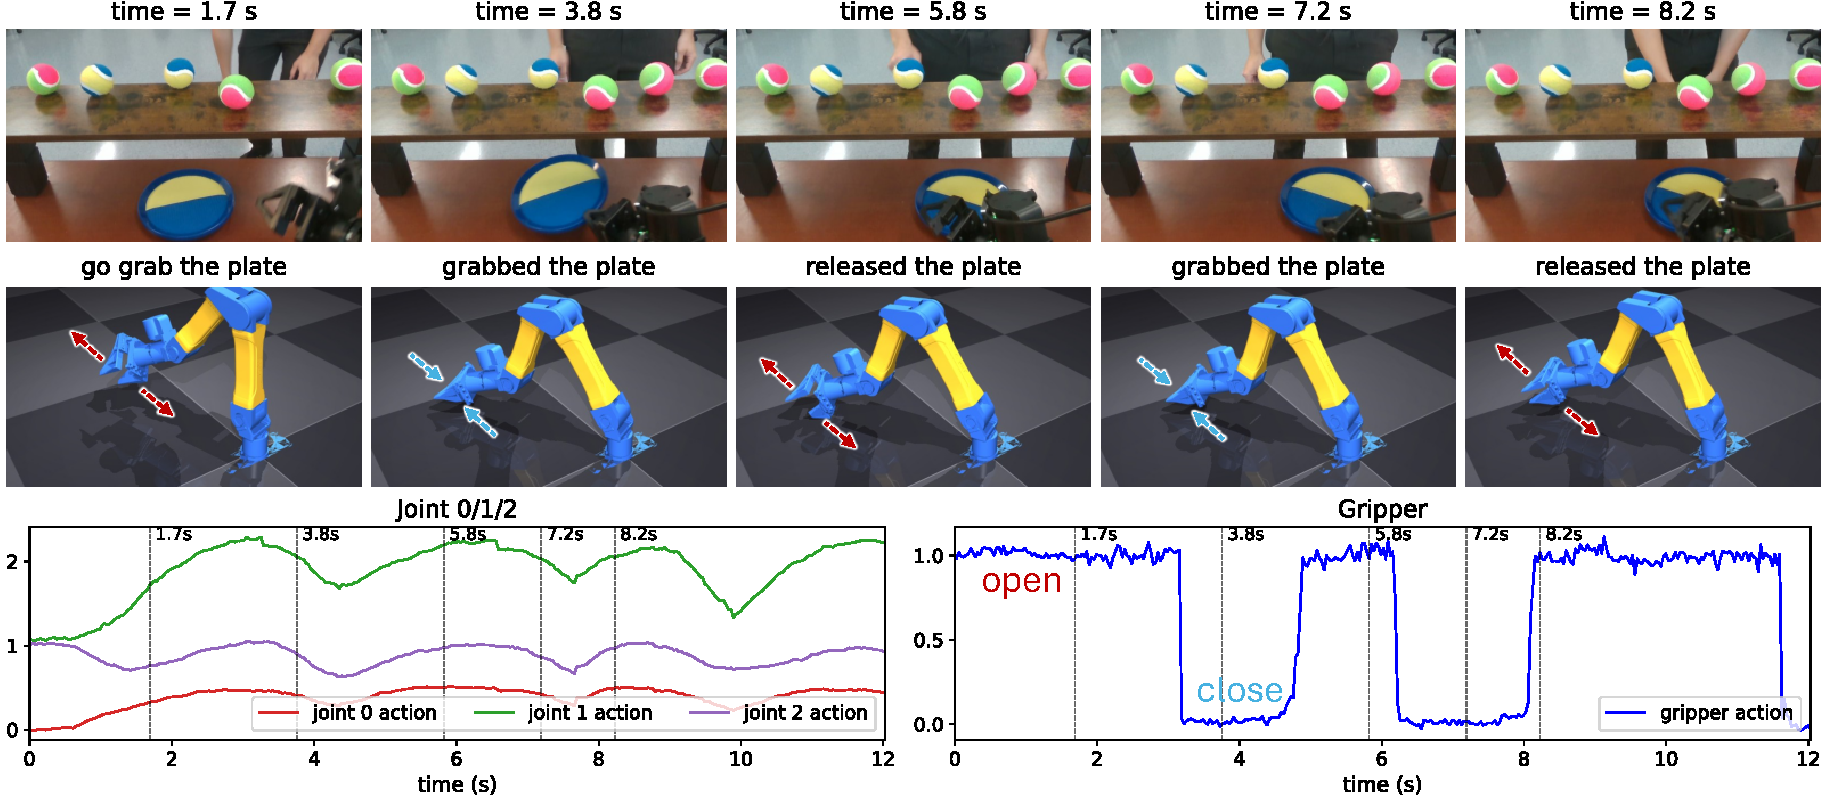
\includegraphics[width=\columnwidth]{2026-corl-unveil-template/figures/state_alias.pdf}
	\caption{\textbf{VLASH rollout on the untrimmed Flick Catch task.} The task is to grip the velcro plate and follow the human hand. VLASH's gripper hovers near the plate without committing to grasp or retract, because a single-frame observation cannot differentiate reaching for the plate from releasing it. RTC exhibits the same failure (see project page).}
	\label{fig:ambiguity}
\end{figure}

Because both baselines collapse to $0\%$ on the untrimmed task, a direct comparison there is uninformative. To enable a non-trivial comparison that isolates motion ambiguity from state aliasing, we manually trim the release-and-retract segment from every episode of the Flick Catch and Wine Pour training and evaluation data; the success rates on this trimmed version are reported in \cref{tab:success_rates}. The trimmed task still requires motion-aware perception (target tracking and timing) but removes the state-aliased segment.

To verify that \ours\ resolves state aliasing rather than merely benefiting from this trimming, we additionally train and evaluate every method on the original, untrimmed episodes. \cref{tab:state_alias} (in \cref{sec:diagnosis}) reports the resulting success rates: RTC and VLASH again fail every rollout, while \ours\ succeeds at $68\%$ on Flick Catch and $97.6$\% on Wine Pour. We attribute the gain to \TEMPOACT: the proprioceptive history distinguishes task phases that the current frame cannot, letting the policy commit to the correct action rather than hedging between reach-out and retract.

\section{Experimental Setup Details}
\label{app:setup}

\emph{Supplements \cref{sec:exp-setup}.}

\subsection{Hardware Platform}
All experiments are conducted on a bimanual workstation consisting of two I2RT YAM Ultra robot arms~\cite{i2rt_yam_ultra}, each with 7 degrees of freedom. The two arms are mounted and clamped to the table edge with their bases separated by 24 inches (61 cm). Both arms are placed on a rigid table measuring 6 ft × 29.5 in × 28 in (width × depth × height; 183 × 75 × 71 cm). Each arm is equipped with a parallel-jaw gripper.

 Visual observations are provided by three cameras: one fixed third-person camera positioned between the two arms and two wrist-mounted cameras. Each camera streams 224p at 30 Hz. Policies are executed at 30 Hz, if possible.

\subsection{Evaluation Protocol}

For the Drop Catch task, a single ball is released above the workspace from a height of 13–18 in (33–46 cm), measured from the table surface to the release point. The ball is tennis-ball sized and covered in a velcro-compatible material so that it adheres to the velcro plate that the gripper holds.

For the Flick Catch task, 5–6 balls are arranged on a shelf measuring 31.5 × 7.9 × 8.5 in (80 × 20 × 21.6 cm; width × depth × height), positioned near the table edge opposite to where the arms are clamped. These balls are identical to the one used in the Drop Catch task.

To ensure a fair evaluation, the human operator releasing the ball performs each trial with eyes closed while wearing headphones, preventing them from anticipating the robot's position and biasing the release point toward it.

\subsection{Training Details}

Each policy is trained on eight NVIDIA RTX PRO 6000 Blackwell GPUs. Training a single policy takes approximately 2 hours. More specifically, with an effective batch size of $128$ the per-iteration time is $0.49$s for VLASH, $0.46$s for RTC, and $0.50$s for \ours. RTC does not have an openly available codebase, so we reimplement it faithfully from its paper.


\section{Per-Task Failure Mode Breakdown}
\label{app:failure_breakdown}

\emph{Supplements \cref{sec:quant} and \figref{fig:failure_modes}.} To complement the Bottle Handover analysis in \cref{sec:quant}~(\figref{fig:failure_modes}), we apply the same protocol to Flick Catch and Drop Catch: we visually examine all $50$ rollouts per method on the trimmed task and assign each to a success or to one failure category. The categories differ across tasks because each task has different failure modes.

\begin{figure}[h]
	\centering
	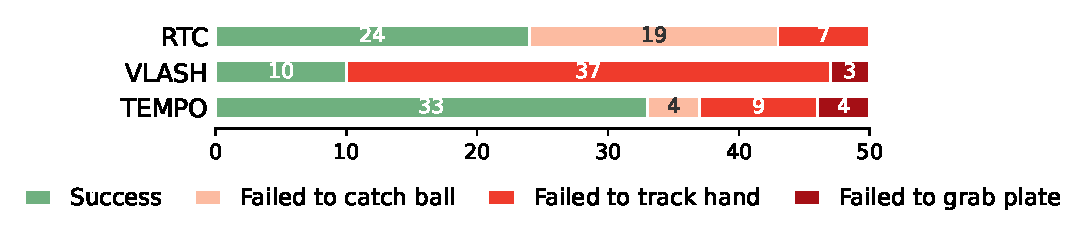
\includegraphics[width=\columnwidth]{2026-corl-unveil-template/figures/failure_modes_flick.pdf}
	\caption{\textbf{Failure-mode breakdown on Flick Catch.} Each of the $50$ rollouts is decomposed into success plus three failure modes corresponding to the three task stages (grab plate, track hand, catch ball). VLASH's failures concentrate in hand-tracking and RTC struggles most at tracking the ball's trajectory (see project page); \ours~cuts both failure modes.}
	\label{fig:flick_failure}
\end{figure}

\paragraph{Flick Catch (\figref{fig:flick_failure}).}
We assign each failed rollout to one of three failure modes corresponding to the three task stages: grabbing the plate, tracking the hand, or catching the flicked ball. VLASH's failures concentrate almost entirely in hand-tracking: in $37$ of $50$ trials the policy fails to follow the human hand and therefore never reaches the catching stage. RTC reacts to the hand but loses the flicked ball, with ball-catch failures accounting for $19$ trials, the dominant mode for RTC. \ours\ cuts VLASH's hand-tracking failures from $37$ to $9$ and RTC's ball-catch failures from $19$ to $4$; the residual failures are spread across all three stages rather than concentrated in any single one.

\begin{figure}[h]
	\centering
	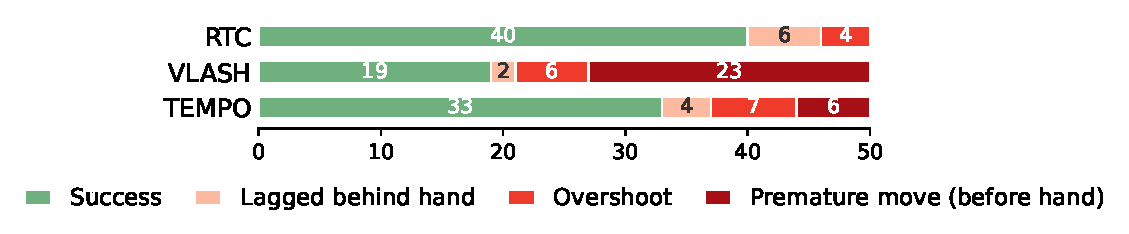
\includegraphics[width=\columnwidth]{2026-corl-unveil-template/figures/failure_modes_drop.pdf}
	\caption{\textbf{Failure-mode breakdown on Drop Catch.} RTC scores highest as Drop Catch is dominated by reactive timing rather than motion or state ambiguity. VLASH's dominant failure is premature movement before the human's hand begins to move; \ours\ cuts this failure by nearly $4\times$.}
	\label{fig:drop_failure}
\end{figure}

\paragraph{Drop Catch (\figref{fig:drop_failure}).}
Drop Catch is the timing-dominated task on which RTC scores highest~(\cref{tab:success_rates}); its only failures are a few overshoots ($4$) and lags ($6$). VLASH, despite also being asynchronous, exhibits a markedly different profile: it \emph{moves before the human's hand} in $23$ of $50$ trials, a near-majority failure that pulls its success rate down to $19$. \ours\ cuts this premature-move failure by nearly $4\times$ (from $23$ to $6$), with only a small change in overshoots ($6\to 7$). The premature-move reduction is consistent with the role of \TEMPOACT: the proprioceptive history records what the policy has already begun, so it does not re-initiate a move on every frame.


\begin{figure}[h]
	\centering    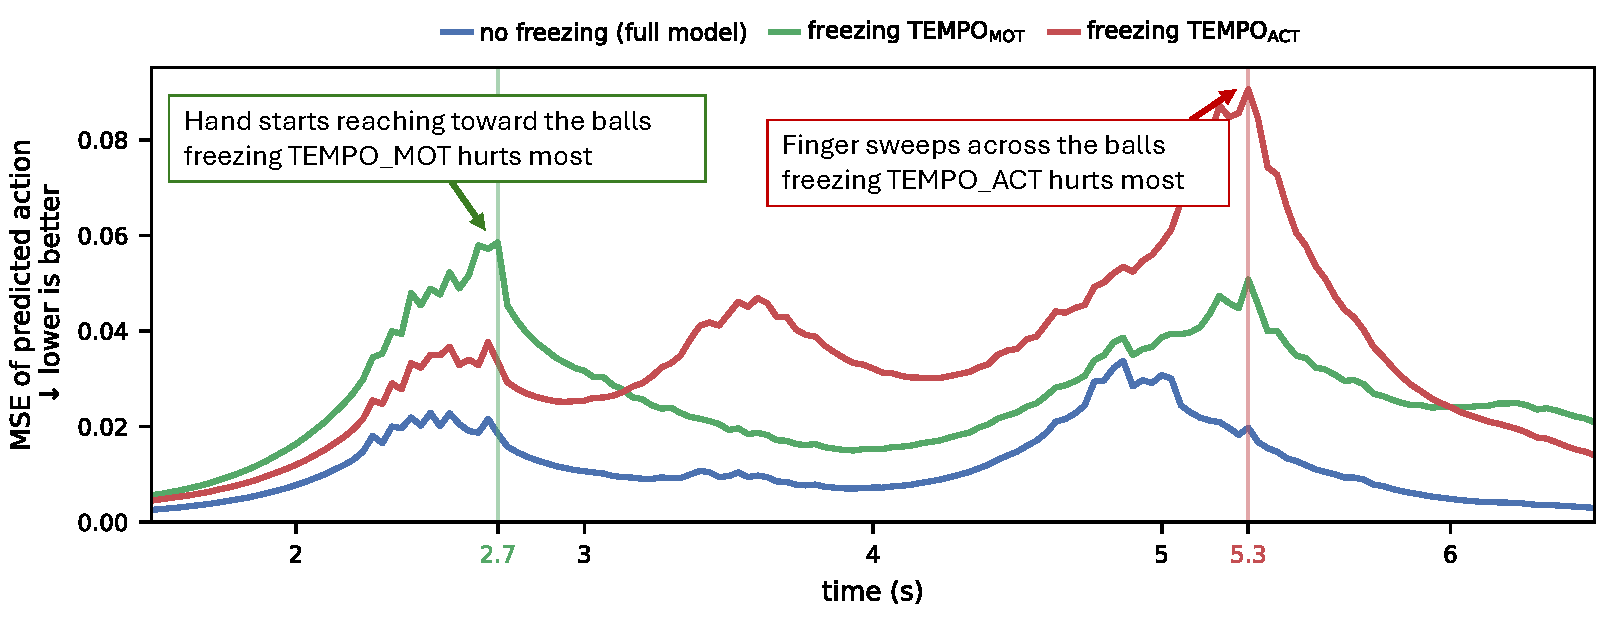
\includegraphics[width=0.9\columnwidth]{2026-corl-unveil-template/figures/ablation_mse.pdf}
	\vspace{-0.6em}
    \caption{\textbf{Both \TEMPOMOT\ and \TEMPOACT\ are necessary.} Per-frame action MSE for the full \ours\ model (blue) vs. the two single-signal ablations, evaluated on the Flick Catch task. Freezing \TEMPOMOT\ to its first-frame value (green) hurts most at $2.7$\,s, the beginning of the task where human hand starts to move. Freezing \TEMPOACT\ (red) hurts most at $5.3$\,s, the middle of the task where the finger sweeps horizontally across the balls before picking one and flicking it. Thus, each signal plays an important role at a different moment in the task.}
	\label{fig:attention_mse}
\end{figure}


\section{Input Ablation}
\label{app:input_ablation}




\emph{Supplements the modality-ablation analysis in \cref{sec:ablation}.}
To test whether \TEMPOMOT\ and \TEMPOACT\ are both necessary and contribute meaningfully to task performance, we run a per-frame ablation on a representative episode of the Flick Catch task (\figref{fig:attention_mse}). For each frame we ``remove'' each input modality by freezing \TEMPOMOT\ or \TEMPOACT\ to its first-frame value and measure the resulting predicted-action MSE; curves are EMA-smoothed for readability. Freezing either modality substantially degrades the policy's action prediction at different points in the episode. Freezing \TEMPOMOT\ hurts most at $2.7$\,s, the beginning of the task where large motions occur: MSE rises from $0.019$ to $0.059$ ($3.1\times$), while freezing \TEMPOACT\ costs only $0.033$. Freezing \TEMPOACT\ hurts most at $5.3$\,s, the middle of the task where the finger sweeps horizontally across the balls before picking one and flicking it, and there the pattern reverses: freezing \TEMPOACT\ hurts more than \TEMPOMOT\ ($0.091$ vs.\ $0.051$; full $0.020$). Each signal helps a different phase of the task.

\section{Motion Encoder Selection}
\label{app:motion_encoder}

\begin{figure}[h]
\centering

% --- Top row: per-task probing targets (image + label tightly coupled per panel) ---
\begin{minipage}[b]{0.235\columnwidth}
	\centering
	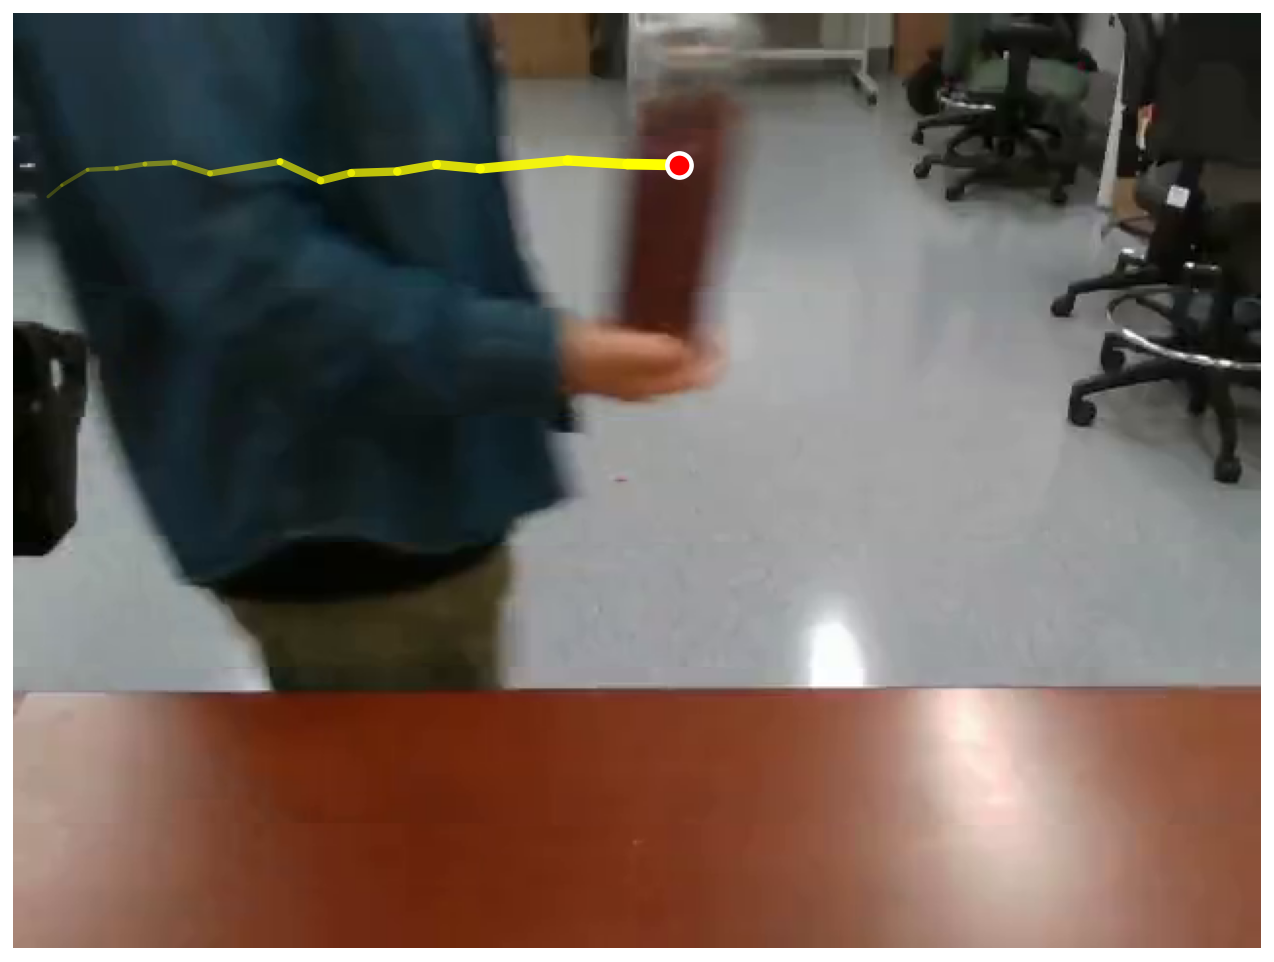
\includegraphics[width=\linewidth]{2026-corl-unveil-template/figures/velocity_handover.png}\\
	{\small Bottle Handover}
\end{minipage}\hfill
\begin{minipage}[b]{0.235\columnwidth}
	\centering
	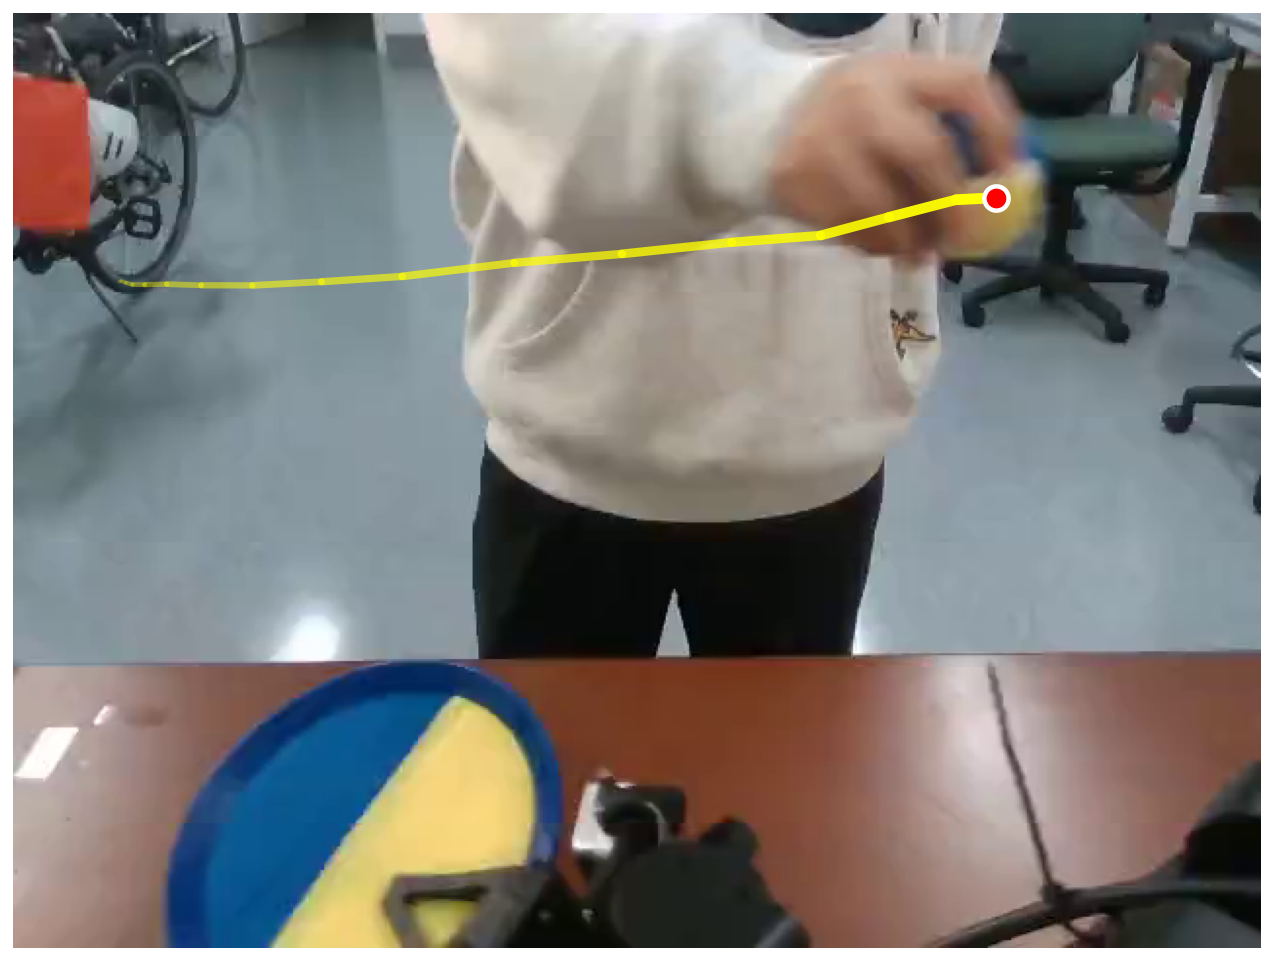
\includegraphics[width=\linewidth]{2026-corl-unveil-template/figures/velocity_drop.png}\\
	{\small Drop Catch}
\end{minipage}\hfill
\begin{minipage}[b]{0.235\columnwidth}
	\centering
	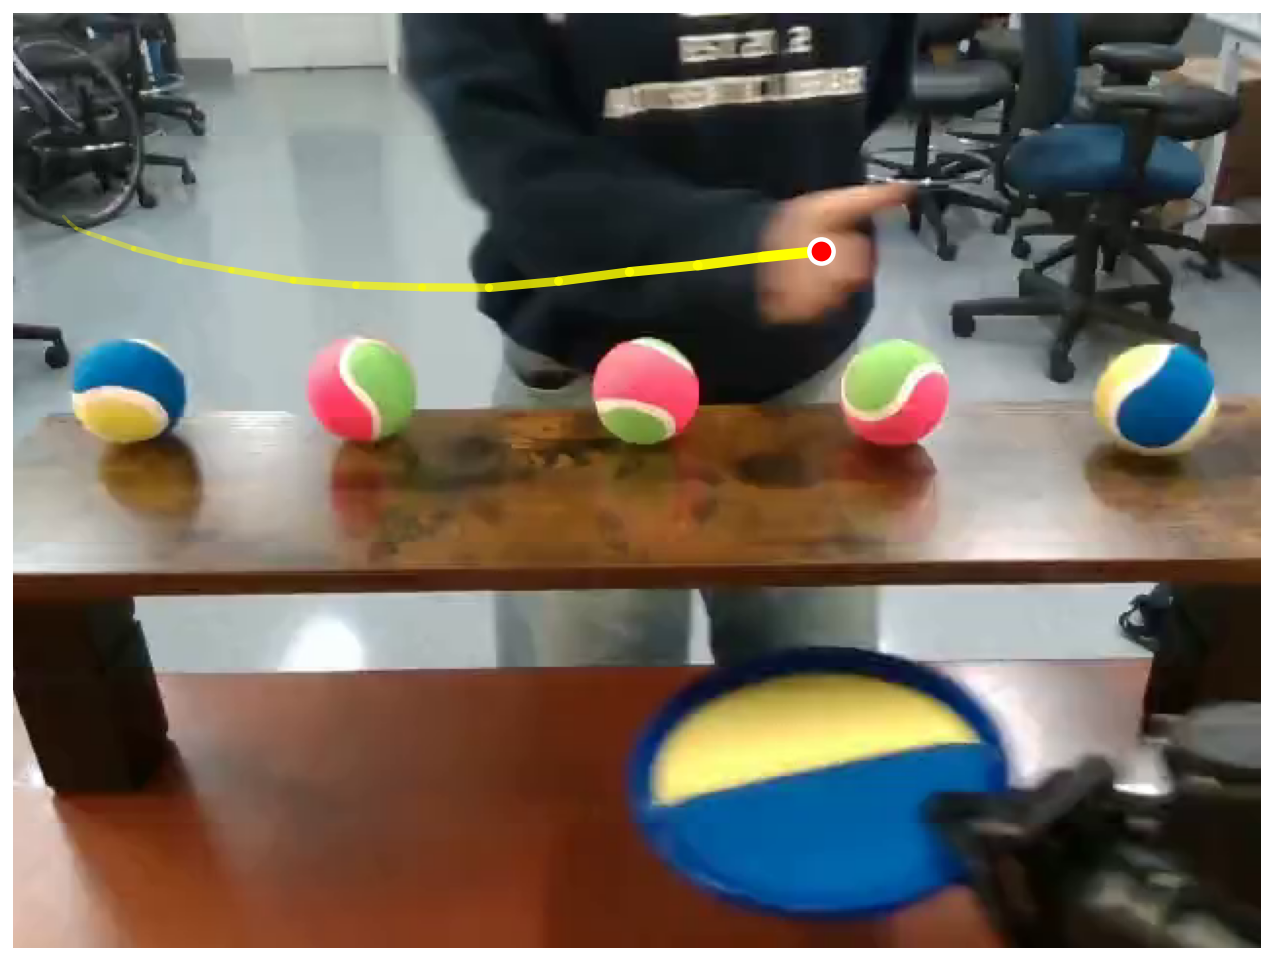
\includegraphics[width=\linewidth]{2026-corl-unveil-template/figures/velocity_flick.png}\\
	{\small Flick Catch}
\end{minipage}\hfill
\begin{minipage}[b]{0.235\columnwidth}
	\centering
	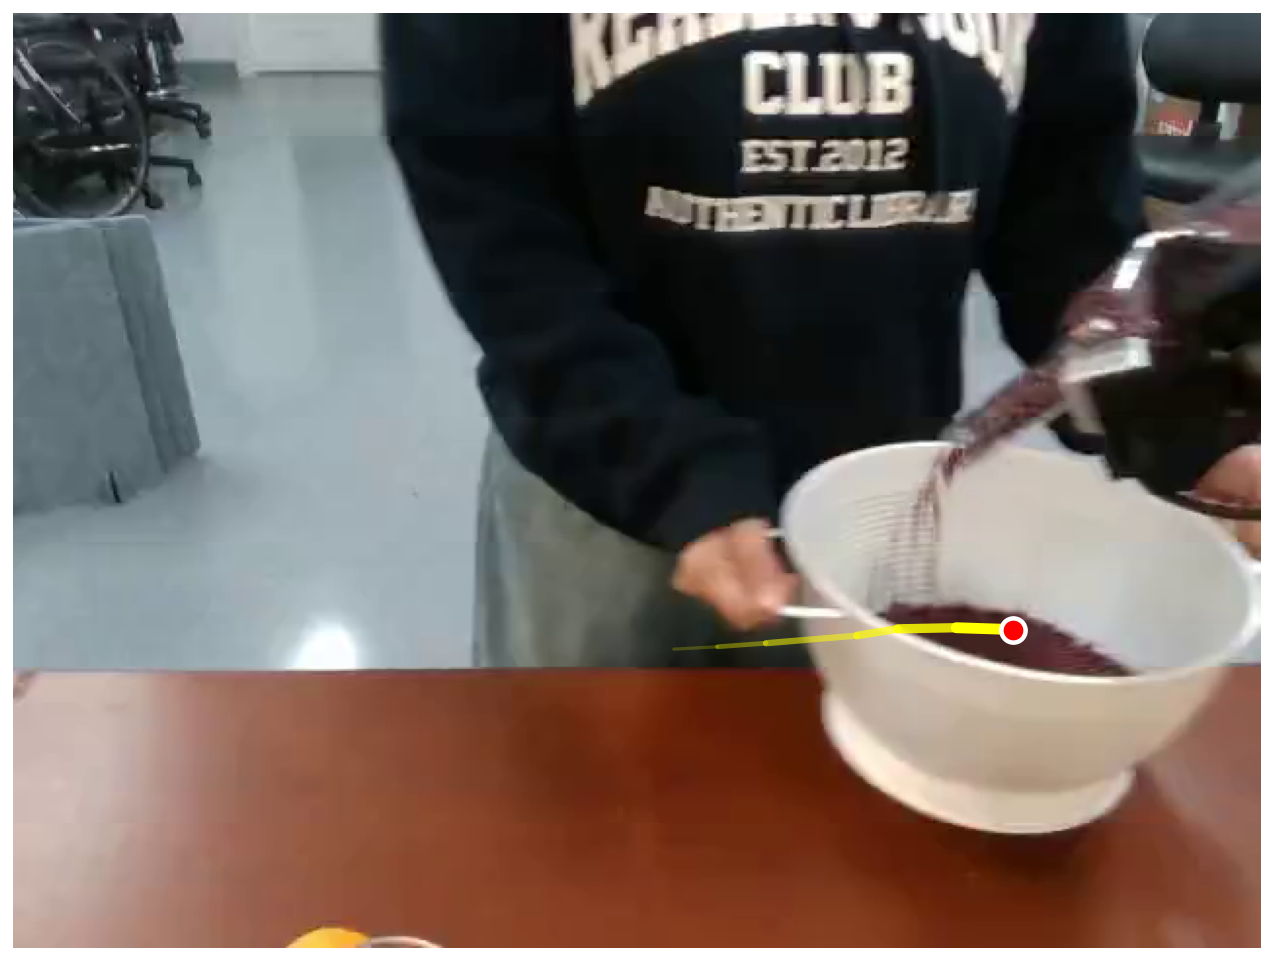
\includegraphics[width=\linewidth]{2026-corl-unveil-template/figures/velocity_pour.png}\\
	{\small Wine Pour}
\end{minipage}

\vspace{8pt}

% --- Bottom: probe results ---
\small
\begin{tabular}{lccccc}
\toprule
\textbf{Initialization for \TEMPOMOT} & \textbf{Bottle Handover} & \textbf{Drop Catch} & \textbf{Flick Catch} & \textbf{Wine Pour} & \textbf{Average} \\
\midrule
% Random                                & -0.01 & 0.00 & 0.00 & 0.00 & 0.00 \\
Object Position                          & 0.24  & 0.03 & 0.03 & 0.02 & 0.08 \\
VideoLaVIT~\cite{videolavit}             & 0.45  & 0.25 & 0.28 & 0.36 & 0.34 \\
Reducio~\cite{reducio}                   & 0.50  & 0.36 & 0.38 & 0.32 & 0.39 \\
SAM~2~\cite{sam2}                        & 0.58  & 0.37 & 0.50 & 0.39 & 0.46 \\
VidTwin~\cite{vidtwin}                   & 0.59  & 0.44 & 0.43 & 0.45 & 0.48 \\
\bottomrule
\end{tabular}

\caption{\textbf{Linear probe of candidate initializations for \TEMPOMOT.} \emph{Top:} one example frame per task showing the object of interest (red dot) and its recent trajectory (yellow line); the pixel-space velocity of this object is the regression target the linear probe must predict. \emph{Bottom:} per-task velocity $R^2$ for each candidate initialization, along with the average. Higher is better; the raw object-position baseline ($R^2=0.08$ on average) cannot recover velocity from a single position, while every learned motion encoder does so substantially better.}
\label{fig:ball_velocity_probe}
\end{figure}


\emph{Supplements the motion-encoder definition in \cref{sec:method} (the $\phi$ in \TEMPOMOT).}
\ours\ is agnostic to the choice of motion encoder; here we justify ours. Reusing the per-frame object-velocity annotation from our motion probe (\secref{sec:analysis}; the per-task probing target is visualized at the top of \figref{fig:ball_velocity_probe}), we fit a \emph{linear} probe from each candidate motion latent to the object's velocity: if the latent captures the object's motion, a linear readout should recover the velocity with high $R^2$. Every learned encoder decodes velocity far above the raw object position (avg.\ $R^2 = 0.08$), confirming that object motion is genuinely present in the latent and that a single position, like a single frame, does not by itself encode meaningful information to infer object motion. SAM~2 and VidTwin score highest; we adopt SAM~2.1-Tiny because it pairs near-top motion correlation with the streaming speed required for real-time deployment (\cref{tab:latency_comparison}).


%===============================================================================

\end{document}
